%!TeX program = xelatex

% Define document font, paper size and type %
\documentclass[11pt,a4paper,numbers=noenddot]{scrreprt}

% Include all auxiliary packages
% All required packages to be used within this project

% Margin definitions
\usepackage[a4paper,vmargin=3cm,hmargin=3cm]{geometry}

% Packages to be used
\usepackage{fontspec}
\usepackage{eurosym}
\usepackage{amssymb}
\usepackage{mathtools}
\usepackage{amsmath}
\usepackage{upquote}
\usepackage{microtype}
\usepackage{longtable,booktabs}
\usepackage{graphicx}
\usepackage{grffile}
\usepackage{appendix}
\usepackage{float}
\usepackage{pst-all}
\usepackage{geometry}
\usepackage{xcolor}
\usepackage{xpatch}
\usepackage{nccmath}
\usepackage{subcaption}
\usepackage{xcolor}
\usepackage{multirow}
\usepackage{setspace}
\usepackage{bm}
\usepackage[
  starfontserif % comment for sans glyphs
]{starfont}
\captionsetup{compatibility=false}
\usepackage[crop=off]{auto-pst-pdf}
\usepackage[normalem]{ulem}

% Custom links color
\definecolor{linkscolor}{rgb}{0.89, 0.26, 0.2}

\usepackage[unicode=true,bookmarks=true,bookmarksopen=false,
  bookmarksopenlevel=1,pdfborder={0 0 0},backref=false,
  colorlinks=true,allcolors=red,pdfstartview=Fit,
  pdfcenterwindow=true,pdfdisplaydoctitle=true,
  pdfpagelayout=OneColumn,linktocpage=true]{hyperref}
\useunder{\uline}{\ul}{}

% Path for all graphic utilities
\graphicspath{{fig/}}



% Bibliography setup
% Style: https://www.overleaf.com/learn/latex/Biblatex_bibliography_styles
% Cite style: https://www.overleaf.com/learn/latex/Biblatex_citation_styles
\usepackage[backend=biber, style=verbose, citestyle=authoryear, sorting=ynt]{biblatex}

% Define how author names are formatted in citations
\DeclareNameAlias{sortname}{family-given}

\bibliography{bib/articles_modern}
\bibliography{bib/books_classic}
\bibliography{bib/books_modern}

% Custom commands: always the last ones to import to properly override default
% Custom paragraph distance
\setlength{\parskip}{1em plus 2pt minus 1pt}
\setlength{\emergencystretch}{3em}

% Beautiful captions for figures
\captionsetup[figure]{
  format=hang,
  name=Fig.,
  singlelinecheck=off,
  labelsep=colon,
  labelfont=bf,
  font=small
}

% Improve quotations
\newcommand{\quoteauthor}[2]
{
  \begin{flushright}
    \rightskip=1.8cm\textit{``{#1}''} \\
    \vspace{.2em}
    \rightskip=.8cm---{#2}
  \end{flushright}
}

% Improve hyperlinks when citing references
\DeclareCiteCommand{\citetitle}
{\boolfalse{citetracker}%
  \boolfalse{pagetracker}%
  \usebibmacro{prenote}}
{\ifciteindex
  {\indexfield{indextitle}}
  {}%
  \printtext[bibhyperref]{\printfield[citetitle]{labeltitle}}}
{\multicitedelim}
{\usebibmacro{postnote}}

\DeclareCiteCommand{\cite}
{\usebibmacro{prenote}}
{\usebibmacro{citeindex}%
  \printtext[bibhyperref]{\usebibmacro{cite}}}
{\multicitedelim}
{\usebibmacro{postnote}}

\DeclareCiteCommand*{\cite}
{\usebibmacro{prenote}}
{\usebibmacro{citeindex}%
  \printtext[bibhyperref]{\usebibmacro{citeyear}}}
{\multicitedelim}
{\usebibmacro{postnote}}

\DeclareCiteCommand{\parencite}[\mkbibparens]
{\usebibmacro{prenote}}
{\usebibmacro{citeindex}%
  \printtext[bibhyperref]{\usebibmacro{cite}}}
{\multicitedelim}
{\usebibmacro{postnote}}

\DeclareCiteCommand*{\parencite}[\mkbibparens]
{\usebibmacro{prenote}}
{\usebibmacro{citeindex}%
  \printtext[bibhyperref]{\usebibmacro{citeyear}}}
{\multicitedelim}
{\usebibmacro{postnote}}

\DeclareCiteCommand{\footcite}[\mkbibfootnote]
{\usebibmacro{prenote}}
{\usebibmacro{citeindex}%
  \printtext[bibhyperref]{ \usebibmacro{cite}}}
{\multicitedelim}
{\usebibmacro{postnote}}

\DeclareCiteCommand{\footcitetext}[\mkbibfootnotetext]
{\usebibmacro{prenote}}
{\usebibmacro{citeindex}%
  \printtext[bibhyperref]{\usebibmacro{cite}}}
{\multicitedelim}
{\usebibmacro{postnote}}

\DeclareCiteCommand{\textcite}
{\boolfalse{cbx:parens}}
{\usebibmacro{citeindex}%
  \printtext[bibhyperref]{\usebibmacro{textcite}}}
{\ifbool{cbx:parens}
  {\bibcloseparen\global\boolfalse{cbx:parens}}
  {}%
  \multicitedelim}
{\usebibmacro{textcite:postnote}}

\DeclareCiteCommand{\citeauthor}%
{\boolfalse{citetracker}%
  \boolfalse{pagetracker}%
  \usebibmacro{prenote}}
{\ifciteindex
  {\indexnames{labelname}}
  {}%
  \printtext[bibhyperref]{\printnames{labelname}}}
{\multicitedelim}
{\usebibmacro{postnote}}

% Reduce top and lower space in equations
\xpatchcmd{\NCC@ignorepar}{%
  \abovedisplayskip\abovedisplayshortskip}
{%
  \abovedisplayskip\abovedisplayshortskip%
  \belowdisplayskip\belowdisplayshortskip}
{}{}

% Do not restart footnotes counter
\counterwithout{footnote}{chapter}

% Custom norm for equations
\DeclarePairedDelimiter{\norm}{\lVert}{\rVert}

% Custom arctan2 and atan2 functions
\DeclareMathOperator{\arctantwo}{arctan2}
\DeclareMathOperator{\atantwo}{atan2}

% Custom piecewise functions
\DeclarePairedDelimiter\Floor\lfloor\rfloor
\DeclarePairedDelimiter\Ceil\lceil\rceil

% Trigonometric functions
\DeclareMathOperator{\sech}{sech}
\DeclareMathOperator{\csch}{csch}
\DeclareMathOperator{\arcsec}{arcsec}
\DeclareMathOperator{\arccot}{arccot}
\DeclareMathOperator{\arccsc}{arccsc}
\DeclareMathOperator{\arccosh}{arccosh}
\DeclareMathOperator{\arcsinh}{arcsinh}
\DeclareMathOperator{\arctanh}{arctanh}
\DeclareMathOperator{\arcsech}{arcsech}
\DeclareMathOperator{\arccsch}{arccsch}
\DeclareMathOperator{\arccoth}{arccoth}

% Custom command for blank page
\newcommand{\blankpage}{\newpage \ \thispagestyle{empty} \newpage}

% Custom command for the table of contents
\newcommand{\maketableofcontents}{\tableofcontents \blankpage \listoffigures \blankpage \listoftables \blankpage}

% Solar System Symbols
\DeclareSymbolFont{starfontsym}{OT1}{sts}{m}{n}
\DeclareMathSymbol{\mathSun}{\mathord}{starfontsym}{115}
\DeclareMathSymbol{\mathMercury}{\mathord}{starfontsym}{102}
\DeclareMathSymbol{\mathVenus}{\mathord}{starfontsym}{103}
\DeclareMathSymbol{\mathTerra}{\mathord}{starfontsym}{76}
\DeclareMathSymbol{\mathvarTerra}{\mathord}{starfontsym}{108}
\DeclareMathSymbol{\mathMoon}{\mathord}{starfontsym}{100}
\DeclareMathSymbol{\mathvarMoon}{\mathord}{starfontsym}{97}
\DeclareMathSymbol{\mathMars}{\mathord}{starfontsym}{104}
\DeclareMathSymbol{\mathJupiter}{\mathord}{starfontsym}{106}
\DeclareMathSymbol{\mathSaturn}{\mathord}{starfontsym}{83}
\DeclareMathSymbol{\mathUranus}{\mathord}{starfontsym}{70}
\DeclareMathSymbol{\mathvarUranus}{\mathord}{starfontsym}{65}
\DeclareMathSymbol{\mathNeptune}{\mathord}{starfontsym}{71}
\DeclareMathSymbol{\mathPluto}{\mathord}{starfontsym}{74}
\DeclareMathSymbol{\mathvarPluto}{\mathord}{starfontsym}{72}


% Start the document
\begin{document}
\onehalfspacing

% Switch off page numbering %
\pagenumbering{Roman}

% Append cover and prologue to actual document %
% Start generating the title page
\begin{titlepage}

  % All content will be centered within this page
  \begin{center}

    % Add cover logo
    \begin{figure}[h]
      \centering
      
\includegraphics[width=\linewidth]{static/banner.png}
    \end{figure}
    \vspace{1cm}

    % Nature of the document
    \textsc{\large
      UNIVERSIDAD INTERNACIONAL DE VALENCIA
    }\\[0.25cm]
    \textsc{\large
      Master in Astronomy and Astrophysics \\
      Academic year 2023-2024
    }\\[1cm]
    \textsc{\large
      \textit{Segunda convocatoria}
    }\\[1.25cm]

    % Title of the essay
    \noindent\rule{\textwidth}{1pt}
    \\[0.25cm]
    {
    % Apply font size and color
    \fontsize{35pt}{35pt}\selectfont
    {
      Interstellar Interceptors. Mission design for rendezvous with objects in hyperbolic orbits.
    }
    }
    \noindent\rule{\textwidth}{1pt}

    \vspace{1.5cm}
    \textsc{\Large
      Jorge Martínez Garrido
    }\\[1.25cm]
    \textsc{\large
      Supervised by:
    }\\[0.25cm]
    \textsc{\large
      Josep M. Trigo-Rodríguez (ICE-CSIC/IEEC) \\
      Eloy Peña-Asensio (Politecnico di Milano)
    }\\[1.5cm]

    \textsc{\large
      April, 2024
    }\\[0.25cm]
    \textsc{\large
      Madrid, Spain
    }\\[0.25cm]

  \end{center}
\end{titlepage}

\blankpage
\chapter*{Abstract}

This research offers a thorough examination of transfer orbits specifically
tailored for intercepting interstellar visitors. Through an exhaustive analysis
of diverse launch scenarios, detailed porkchop plots are crafted to illustrate
the specific energy required at launch for both prograde and retrograde
transfers. Additionally, isolines delineating the total time of flight and
velocity upon arrival are meticulously calculated across a broad spectrum of
launch and arrival dates. These efforts enable the precise determination of
optimal energy transfer paths. Departure strategies from Earth, Lagrange point
L2, and gravity-assisted maneuvers are thoroughly explored, providing insights
into their efficacy.

The study's outcomes harmonize with established mission proposals, exemplified
by the Comet Interceptor, corroborating the strategic significance of Lagrange
point L2 as a launch locus for interstellar missions. This underscores the
imperative for enhancing surveillance research initiatives centered on
identifying interlopers and fortifying pre-planned missions stationed at
Lagrange point L2. Given the validated efficacy of L2 as a launch platform,
heightened emphasis on surveillance research emerges as essential, ensuring
preparedness to capitalize on evolving opportunities for celestial exploration
and scientific inquiry.


\vspace{4cm}
\textbf{Keywords:} Interlopers, transfer orbits, porkchop plots, Lagrange points,
gravity-assisted maneuvers, interstellar missions, surveillance research,
mission design, celestial exploration

\blankpage

% Start the table of contents, figures and tables %
\maketableofcontents

% ---------- BEGIN OF CONTENT FILES -------------

% --------------------------------- %
% --- INTRODUCTION TO THIS WORK --- %
% --------------------------------- %
\chapter{Introduction to this work}
\pagenumbering{arabic}

The initial chapter is dedicated to introducing fundamental concepts pertinent
to the addressed problem, delineating the various methodologies employed and
outlining the objectives attained. These components serve to enhance the
reader's comprehension of the project's framework. Furthermore, the concluding
sections offer a compilation of real-world applications alongside a concise
socioeconomic evaluation, aiming to substantiate the contemporary relevance and
significance of the problem at hand.

% --- Sections for this chapter --- %
\section{Problem description and motivation}

The discovery of interstellar objects such as 'Oumuamua and Borisov within our
solar system has ignited a surge of curiosity and scientific interest. These
sub-kilometer-sized visitors, originating from distant stellar systems, present
a unique opportunity to study extraterrestrial bodies that have traversed vast
cosmic distances. Therefore, the main motivation behind the study of these
objects are:

\begin{itemize}

  \item \textbf{Better understanding the formation of planetary systems.}
        Interstellar objects can provide insights into the formation and
        dynamics of planetary systems beyond our own. This could help to
        confirm or reject the Nebular hyphotesis, which is the most popular
        model proposed for the formation of planetary systems.

  \item \textbf{Exploring the origins of life.} Analyzing the composition of
        interstellar objects could provide valuable information about the
        chemical and physical conditions present in other planetary
        systems, shedding light on the origins of life in the universe, which
        could support or reject the panspermia hyphotesis.

  \item \textbf{Technological innovation.} By pushing the technological
        boundaries of space exploration, missions to intercept interstellar
        objects could lead to the development of new propulsion systems and
        spacecraft capable of reaching unprecedented speeds and distances.

\end{itemize}

Given their exceptionally high eccentricities, heliocentric velocities, and
fleeting passage through the planetary region, there is a pressing need for the
development of ready-to-launch missions capable of intercepting them.

However, the design of such missions is not straightforward. The high velocities
of these objects, combined with their limited observation windows, make it
difficult to accurately predict their trajectories and plan for rendezvous
within the short timeframes available.

This problem presents the main motivation of this work: \textbf{devising mission
orbits capable of intercepting interstellar objects}.

This research stems from the desire to unlock the mysteries surrounding these
enigmatic interstellar travelers, gathering invaluable data or even returning
samples from their surfaces. This pursuit not only promises to broaden our
understanding of celestial dynamics and planetary formation but also holds
profound implications for the future of space exploration and our comprehension
of the broader universe.

\section{Objectives and goals}

The main objetive of this project is to devise suitable targetting orbits for
interstellar ojects. To achieve this purpose, the whole process is divided
into the following key objectives:

\begin{itemize}

    \item \textbf{Research on interstellar objects.}
        The definition of interstellar object is presented together with the
        official IAU nomenclature. The only two discovered objects,
        'Oumuamua and Borisov, are presented together with their main
        characteristics. The importance of the solar apex is explained
        too.

    \item \textbf{Research on targetting orbits.}
        The main types of targetting orbits are presented, together with their
        main characteristics. The main differences between them are explained
        and the main advantages and disadvantages of each type are presented.

\end{itemize}

\section{Social and economic impact}

Public scrutiny often targets science funding, demanding evidence of its
tangible social and economic benefits. This challenge is particularly pronounced
in fields like astronomy and astrodynamics, where justifying investments for
exploring distant celestial objects and phenomena is difficult.

A pivotal outcome of the research process lies in the array of technologies
conceived, subsequently finding diverse applications for societal improvement.
Consider the iconic Apollo program as an example. The groundbreaking
technologies developed for the success of Apollo missions, including the
formidable Saturn V rocket, the versatile Lunar Module, and the pioneering
Apollo Guidance Computer (AGC) depicted in Figure \ref{fig:apollo-agc}, have
transcended their original purposes and found invaluable utility across various
fields.

\begin{figure}[H]
  \centering
  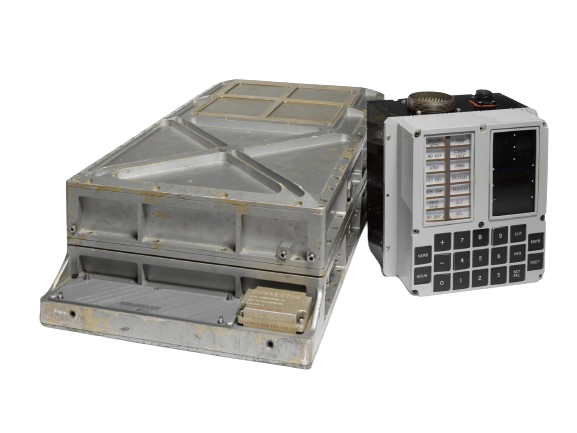
\includegraphics[width=0.7\textwidth]{static/apollo-agc.png}
  \caption[Apollo Guidance Computer]{
  The figure displays two key components of the AGC: the Computer Unit,
  constructed entirely from NOR gate integrated circuits on the left, and
  the Display and Keyboard (DSKY) on the right, used by astronauts to
  interact with the AGC.
  }
  \label{fig:apollo-agc}
\end{figure}

These technologies incorporated novel approaches, notably the utilization of
integrated circuits (ICs). The challenges addressed during this era have paved
the way for modern advancements, evident in the widespread adoption of
fly-by-wire technology in commercial airplanes and the ubiquitous presence of
ICs in various devices.

Similarly, the study of interstellar objects holds promise for fostering
innovation in propulsion, navigation, and observation technologies. These
advancements can be subsequently adapted and applied in other disciplines, such
as Earth observation, satellite communications, and space debris mitigation.


\chapter{Review of interstellar objects}

This chapter is devoted to the 





% --- Sections for this chapter --- %
\section{Definition, origin, abundance, and other attributes}

This section provides a brief overview of interstellar objects. For a deeper
review on interstellar objects, the reader is referred to \cite{jewitt2023},
whose 

% Definition
Interstellar objects (ISOs) are asteroids, comets planets moving through
interstellar medium (ISM) without being gravitationally bound to a star.
Eventually, ISOs can pass through a planetary system, such as the solar system.
Some of them may be even captured.

ISOs are also referred to as interstellar interlopers \cite{jewitt2023}, as they
can be seen as intruders travelling through a different system from their
original one.

% Origin
There are different mechanisms that can lead to the ejection of ISOs from their
original system. The most common are:

\begin{itemize}
    \item \textbf{Stellar encounters}: ISOs can be ejected from their original
          system due to gravitational interactions with other stars. This
          mechanism is particularly relevant in dense stellar environments, such
          as globular clusters, see \cite{portegies2018}.
            
    \item \textbf{Planetary encounters}: Planetary encounters can also lead to
        the ejection of ISOs. This mechanism is particularly relevant in
        planetary systems with large planets, such as Jupiter and Saturn, see
        \cite{kaib2011}.
          
    \item \textbf{Stellar explosions}: Supernovae and other stellar explosions
        can also lead to the ejection of ISOs. These events can provide the
        necessary energy to eject ISOs from their original system, see
        \cite{portegies2018}.
\end{itemize}

% Abundance
The abundance of ISOs in the galaxy is still an open question due to the lack of
enough data to make a reliable estimation. This lack of data has lead
researchers to generate synthetic populations of ISOs to estimate density
limits. Table \ref{tab:iso_density_limits} shows the density limits estimated
by different studies:

% Table with the following values
% Gaidos 2017: 1.0e+14 1 / pc3 = 1.1e-02 1 / AU3
% Jewitt 2017: 8.0e+14 1 / pc3 = 9.1e-02 1 / AU3
% Portegies 2018: 1.0e+14 1 / pc3 = 1.1e-02 1 / AU3
% Feng 2018: 4.8e+13 1 / pc3 = 5.5e-03 1 / AU3
% Fraser 2018: 8.0e+14 1 / pc3 = 9.1e-02 1 / AU3
% Do 2018: 2.0e+15 1 / pc3 = 2.3e-01 1 / AU3

\begin{table}[H]
    \centering
    \begin{tabular}{|c|c|c|}
        \hline
        \textbf{Study} & \textbf{Density limit ($1/\text{pc}^3$)} & \textbf{Density limit ($1/\text{AU}^3$)} \\
        \hline
        \cite{gaidos2017} & $1.0 \times 10^{14}$ & $1.1 \times 10^{-02}$ \\
        \cite{jewitt2017} & $8.0 \times 10^{14}$ & $9.1 \times 10^{-02}$ \\
        \cite{portegies2018} & $1.0 \times 10^{14}$ & $1.1 \times 10^{-02}$ \\
        \cite{feng2018} & $4.8 \times 10^{13}$ & $5.5 \times 10^{-03}$ \\
        \cite{fraser2018} & $8.0 \times 10^{14}$ & $9.1 \times 10^{-02}$ \\
        \cite{do2018} & $2.0 \times 10^{15}$ & $2.3 \times 10^{-01}$ \\
        \hline
    \end{tabular}
    \caption{Density limits estimated by different studies. Note that future
    discoveries and improvements in detection techniques can lead to different
    estimations. Adapted from \cite{moro2023}.}
    \label{tab:iso_density_limits}
\end{table}






% ARTILCES
% file:///home/jorge/Downloads/Moro-Mart%C3%ADn_2009_ApJ_704_733.pdf
% file:///home/jorge/Downloads/Interstellar_Planetesimals_Potential_Seeds_for_Pla.pdf
% Synthetic population: https://arxiv.org/pdf/2301.09375.pdf





As the solar system moves within the Local Interstellar Cloud (LIC), also
referred to as the Local Fluff, interstellar materials penetrates the
heliosphere\footnote{The heliosphere is the region of space dominated by the
Sun's influence. It extends beyond the orbit of Pluto and presents a drop shape
with its tail in the opposite direction of motion of the solar system through
the LIC.} at a rate of $26\text{km/s}$ \cite{hajdukova2020}. These interstellar
materials present a variety of sizes ranging from a few micrometers up to a few
hundreds of meters. Depending on their size and composition, they are subjected
to different forces, such as radiation pressure, solar wind, and the
gravitational pull of the Sun and planets.

\cite{sterken2012} defines the parameter $\beta$ as the ratio between radiation
force and gravity force:

\begin{equation}
    \beta = \frac{|\bm{F_{\text{rad}}}|}{|\bm{F_{\text{G}}}|} = \frac{A_p Q_{pr} S_0}{cG M_{0} m_p}
    \label{eq:deflection_parameter}
\end{equation}

Equation \ref{eq:deflection_parameter} shows that $\beta$ is a function of the
geometric albedo of the particle $A_p$, the radiation pressure coefficient $Q_{pr}$,
the solar constant $S_0$, the speed of light $c$, the gravitational constant $G$,
the solar mass $M_0$, and the particle mass $m_p$.

Three different regimes can be identified according to the value of $\beta$:

\begin{itemize}
    \item $\beta \gg 1$: Radiation pressure dominates over gravity. In this case,
          the particle follows a hyperbolic orbit away from the Sun.
    \item $\beta \sim 1$: Radiation pressure and gravity are comparable. In this
          case, the particle follows a rectilinear orbit towards the sun. Note
          that this is an ideal scenario and small perturbations in both
          forces can lead to a non-linear trajectory.
    \item $\beta \ll 1$: Gravity dominates over radiation pressure. In this
          scenario, gravity dominates and the particle falls towards the Sun in an
          hyperbolic orbit.
\end{itemize}

% TODO: attach figure to show deflection of particles

The heliosphere acts as a shield that protects the solar system from the ISM. It
can deflect small particles. However, larger ISOs can bypass the heliosphere
and enter the solar system.

Discretizing whether a body is an ISO is a challenging task. This is
particularly true for small objects, which are harder to detect and track,
leading to larger measurement errors. 

The following attributes can indicate the interstellar nature of an object:

\begin{itemize}
    \item \textbf{Hyperbolic orbit}: ISOs present hyperbolic orbits since they
          are not gravitationally bound to the Sun. This translates into
          eccentricities greater than the unity.
    \item \textbf{High relative velocity}: ISOs present high relative velocities
          with the planets and other solar system bodies. This is a consequence
          of their interstellar origin.
    \item \textbf{High inclination}: The plane of the solar system is well
          defined by the planets and other bodies. Thus, a body with a high
          inclination and an hyperbolic orbit is likely to be have an
          interstellar origin.
\end{itemize}

Note that these attributes are not exclusive to ISOs. For example, a body with a
high inclination and a hyperbolic orbit could be a comet from the Oort
cloud\footnote{ Oort cloud is a trans-Neptunian region that extends from 2000 to
50000 AU. It is the source of long-period comets and believed to contain a total
mass of 5 Earth masses made up to $10^{12}$ - $10^{14}$ objects. }. However,
studies \cite{francis2005} show that it is more likely that comets originated in the Oort cloud are
ejected into the ISM. Estimations indicate that the ratio between expelled and
retained comets ranges between $\eta = \frac{\text{Comets
expelled}}{\text{Comets retained}} = 3 \text{ - } 100$.

% TODO: **interstellar impostors** oorts cloud objects that resemble to interstellar objects
% TODO: review https://academic.oup.com/mnras/article/492/1/268/5621505?login=false
% https://www.sciencedirect.com/science/article/pii/S0019103523004232

\section{Naming}

The naming of interstellar objects is imposed by the International Astronomical
Union (IAU). The IAU has established a nomenclature for interstellar objects,
which must follow the format\footnote{Exceptions exist. Identifiers may include
the name of the discoverers or even popular names due to legacy reasons.}:

\begin{center}
    [Prefix]/[Year][Half-month][Number]
\end{center}

\textbf{Prefix} is a letter indicating the nature of the object according to
table \ref{tab:iau_prefixes}. Once the interstellar nature has been confirmed,
the prefix sticks to I.

\begin{table}[H]
    \centering
    \begin{tabular}{|c|c|}
        \hline
        \textbf{Object} & \textbf{Prefix} \\
        \hline
        Comet & C \\
        Periodic comet & P \\
        Unknown orbit comet & X \\
        Dissapeared comet & D \\
        Interstellar object & I \\
        \hline
    \end{tabular}
    \caption{IAU prefixes for comets and interstellar objects.}
    \label{tab:iau_prefixes}
\end{table}

\textbf{Year} matches the number of the year of discovery while
\textbf{half-month} is a letter indicating the period of the year when the
discovery was made according to table \ref{tab:iau_half_month_id}.

\begin{table}[H]
    \centering
    \begin{tabular}{|c|c||c|c|}
        \hline
        \textbf{Latin Letter} & \textbf{Half-Month} & \textbf{Latin Letter} & \textbf{Half-Month} \\
        \hline
        A & Jan. 1-15 & B & Jan. 16-31 \\
        C & Feb. 1-15 & D & Feb. 16-29 \\
        E & Mar. 1-15 & F & Mar. 16-31 \\
        G & Apr. 1-15 & H & Apr. 16-30 \\
        J & May 1-15 & K & May 16-31 \\
        L & June 1-15 & M & June 16-30 \\
        N & July 1-15 & O & July 16-31 \\
        P & Aug. 1-15 & Q & Aug. 16-31 \\
        R & Sep. 1-15 & S & Sep. 16-30 \\
        T & Oct. 1-15 & U & Oct. 16-31 \\
        V & Nov. 1-15 & W & Nov. 16-30 \\
        X & Dec. 1-15 & Y & Dec. 16-31 \\
        \hline
    \end{tabular}
    \caption[IAU half-month identifier.]{IAU half-month identifier.}
    \label{tab:iau_half_month_id}
\end{table}

Finally, the \textbf{Number} is the digit representing the order of discovery
within the half-month of discovery. This number starts at $1$ for the first
discovered object of the half-month.

\section{Discovered objects}

In 2017 the first interstellar object was discovered. Initially designated as
1I/2017 U1, this object is now commonly referred to as 1I/'Oumuamua.
Subsequently, in 2019, the discovery of the second interstellar object occurred.
Initially thought to be a comet, it was named C/2019 Q4. Upon confirming its
interstellar nature, this object became known as 2I/Borisov.

Despite originating from the same interstellar realm, both objects exhibited
distinct properties. These unique characteristics are thoroughly examined and
discussed in the subsequent subsections. For a more comprehensive analysis of
these objects and their attributes, reader is encouraged to refer to the work
by \cite{jewitt2022}.

\subsection{1I/'Oumuamua}

'Oumuamua was initially spotted on October 19, 2017, by the Pan-STARRS1
telescope in Hawaii. Initially designated as a comet under the identifier C/2017
U1, it was later reclassified as an asteroid. Figure \ref{fig:oumuamua_orbit}
shows the orbit of this interloper at the moment of its discovery.

\begin{figure}[H]
  \centering
  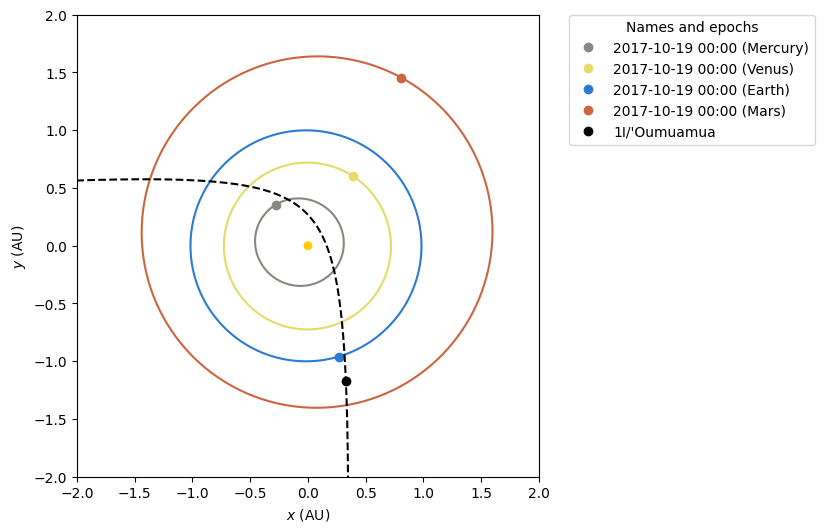
\includegraphics[width=0.95\textwidth]{static/oumuamua/orbit.png}
  \caption[Orbit of 1I/'Oumuamua through the solar system]{
    Orbit of 1I/'Oumuamua through the solar system at the time when it was
    discovered. The interloper presented a perihelion distance of 0.25 AU,
    closer than Mercury. 'Oumuamua exhibits a retrograde orbit.
  }
  \label{fig:oumuamua_orbit}
\end{figure}

'Oumuamua's orbit was calculated to be highly eccentric, with an eccentricity of
$1.20$, indicating a hyperbolic trajectory. Its velocity was estimated to be
approximately $26.0$ km/s. Upon entering the solar system, it approached from
the direction $\alpha_{\text{ICRS}},\; \delta_{\text{ICRS}} = 279^\circ.804,\;
+33^\circ.997$, displaying an inclination significantly deviating from the solar
system's invariant plane and closely aligning with the solar apex, as discussed
in \cite{mamajek2017}. These characteristics collectively suggest an
interstellar origin, as elucidated in subsection
\ref{sec:expected_orbit_attributes}. Table \ref{tab:oumuamua_elements} provides
a summary of 'Oumuamua's orbit elements as of November 23, 2017.

\begin{table}[H]
  \centering
  \begin{tabular}{|c|c|}
    \hline
    Element & Value \\
    \hline
    Eccentricity ($e$) & 1.20 \\
    Semi-major axis ($a$) & -1.27 au \\
    Perihelion ($q$) & 0.26 au \\
    Inclination ($i$) & 122.74 deg \\
    Longitude of the ascending node ($\Omega$) & 24.59 deg \\
    Argument of perihelion ($\omega$) & 241.81 deg \\
    Mean anomaly ($M$) & 51.16 deg \\
    Mean motion ($n$) & 0.69 deg/d \\
    Time of perihelion passage ($T_p$) & 2017-Sep-09.50732138 \\
    \hline
  \end{tabular}
  \caption{Orbit elements of 1I/'Oumuamua as provided by the NASA SBDB.}
  \label{tab:oumuamua_elements}
\end{table}

Surprisingly, this first discovered ISO presented a non-gravitational
acceleration that could not be attributed to cometary properties. In addition,
observations could not determine jetting of particles, an effect experienced by
cometary objects.

'Oumuamua's shape was also a matter of debate. Due to its size, the interloper
appeared as a single point in all telescope images, like the one reproduced in
figure \ref{fig:oumuamua_shape}. At first, it was estimated to have a cigar-like
body. However, later studies solved the best fititng shape that matched the
observed lightcurves. The results indicate that 'Oumuamua should have a planar
disk shape, see \cite{seligman2022}.

\begin{figure}[H]
  \centering
  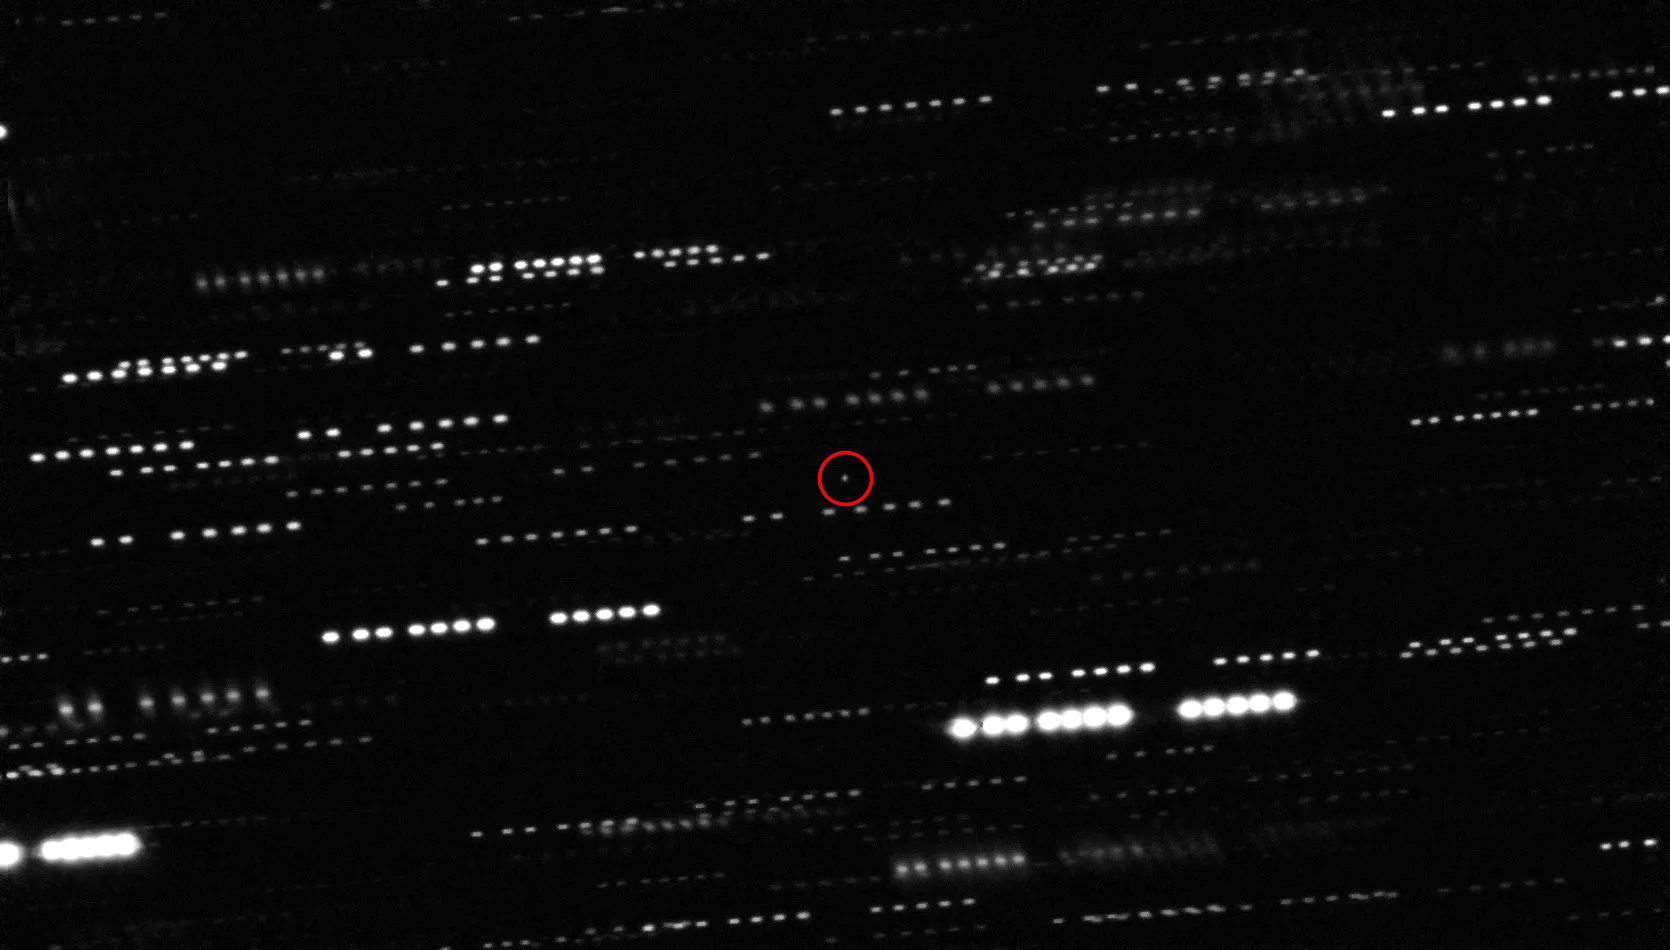
\includegraphics[width=0.95\textwidth]{static/oumuamua/shape.png}
\caption['Oumuamua as seen by the ESO's VLT and GST telescopes]{
  1I/'Oumuamua as seen by the ESO's Very Large Telescope and the Gemini South
  Telescope. This image was released on September 9, 2023. It shows a
  combination of images taken by the two telecopes. The object is seen as
  a point in the center of the image. Background stars are seen as streaks
  due to the telescope's tracking of the object. No cometary tail or mass
  ejection is observed, raising questions about the non-gravitational
  acceleration presented by the interloper.
  }
  \label{fig:oumuamua_shape}
\end{figure}

Unfortunately, 'Oumuamua was discovered after its pasage through the perihelion
and could only be observed for about four weeks before becoming to faint. This
limited the amount of data that could be gathered about the object, increasing
the mistery about the first interstellar object.

\subsection{2I/Borisov}

Borisov was first sighted on August 30, 2019, by Gennady
Borisov\footnote{Borisov, an amateur astronomer from Crimea, detected the second
interloper using his home-built 0.65 meters telescope.}. Initially labeled as a
comet bearing the identifier C/2019 Q4, it underwent reclassification as an
interstellar object subsequent to the determination of its remarkably high
eccentricity. Figure \ref{fig:borisov_orbit} shows the orbit of this interloper
at the moment of its discovery.

\begin{figure}[H]
  \centering
  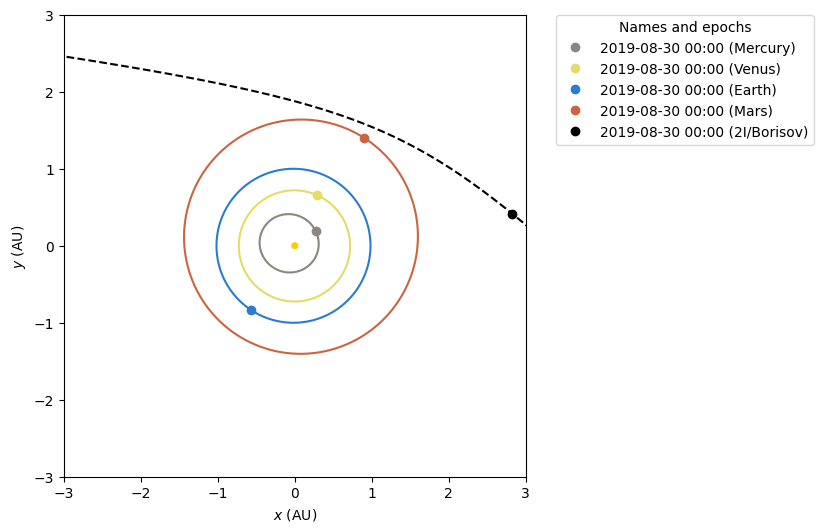
\includegraphics[width=0.95\textwidth]{static/borisov/orbit.png}
  \caption[Orbit of 2I/Borisov through the solar system]{
    Orbit of 2I/Borisov through the solar system. Its eccentricity is
    close to 3.36, making it the most eccentric object observed up to date
    and discarding the possibility of being gravitationally bounded to the Sun.
    Borisov presented a perihelion distance of 2.01 AU, closer than Mars.
  }
  \label{fig:borisov_orbit}
\end{figure}

With an eccentricity of $3.36$ and a velocity of $32.2$ km/s, Borisov exhibited
a hyperbolic orbit. Its inclination of $44.1$ degrees incoming from
constellation Cassiopeia further confirmed its ISO nature. Table
\ref{tab:borisov_elements} provides a summary of Borisov's orbit elements as of
August 1, 2020.

\begin{table}[H]
  \centering
  \begin{tabular}{|c|c|}
    \hline
    Element & Value \\
    \hline
    Epoch ($t$) & August 1, 2020 \\
    Eccentricity ($e$) & 3.36 \\
    Semi-major axis ($a$) & -0.85 au \\
    Perihelion ($q$) & 2.01 au \\
    Inclination ($i$) & 44.05 deg \\
    Longitude of the ascending node ($\Omega$) & 308.15 deg \\
    Argument of perihelion ($\omega$) & 209.12 deg \\
    Mean anomaly ($M$) & 296.54 deg \\
    Mean motion ($n$) & 1.25 deg/d \\
    Time of perihelion passage ($T_p$) & 2019-Dec-08.54507021 \\
    \hline
  \end{tabular}
  \caption{Orbit elements of 2I/Borisov as provided by the NASA SBDB.}
  \label{tab:borisov_elements}
\end{table}

Unlike 'Oumuamua, Borisov displayed a cometary tail. Remarkably, the NASA/ESA
Hubble Space Telescope captured images of this interloper, as depicted in figure
\ref{fig:borisov_shape}.

Analysis revealed that the coma of 2I/Borisov contained significantly more
carbon monoxide (CO) gas than water (H2O), with abundances exceeding 173\%,
surpassing typical cometary compositions within our solar system by over
threefold. Additionally, hydrogen cyanide (HCN) was also detected in the gas
expelled by the comet, with levels comparable to those observed in other solar
system comets \cite{bodewits2020}.

\begin{figure}[H]
  \centering
  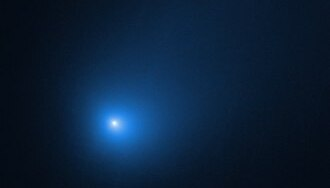
\includegraphics[width=0.95\textwidth]{static/borisov/shape.jpg}
\caption[Borisov as seen by the NASA/ESA Hubble Space Telescope]{
  2I/Borisov as seen by the NASA/ESA Hubble Space Telescope. This image was
  released on December 12, 2019, when the interloper was close to the Sun. Its
  cometary properties are evident in this image. Borisov's tail is seen as a
faint streak extending from the object. It is believed that the tail is composed
of 
  }
  \label{fig:borisov_shape}
\end{figure}

\subsection{Other interstellar candidates}

The interest in interstellar objects has lead a research on previously
discovered objects, in particular interstellar meteors (IM). Interstellar
meteors are meter-scale objects that collide with Earth from a trajectory that
is gravitationally unbound to the Sun, meaning they originate from outside our
solar system. 

Two confirmed interstellar meteors have been identified so far:

\begin{itemize}
  \item CNEOS 2014-01-08 (also known as IM1 or the Manus Island fireball), which
    was detected in 2014 and confirmed as interstellar in 2022 by the U.S. Space
    Command.
  \item CNEOS 2017-03-09 (also known as IM2), which was discovered in 2022 and is
    estimated to have been 10 times more massive than IM1, around 1 meter in
    size.
\end{itemize}

Both IM1 and IM2 were moving at extremely high speeds relative to the local
standard of rest - IM1 at 60 km/s and IM2 at 40 km/s. This high velocity is a
key indicator of their interstellar origin. Analysis of the meteors' material
strength suggests they were tougher than typical iron meteorites, implying they
may not have originated from a planetary system like our own. Plans are underway
to try and retrieve fragments of these interstellar meteors for further study,
which could provide important insights into their composition and origins, see
\cite{siraj2022discovery}.

\section{The role of the solar apex}

% References: http://burro.cwru.edu/Academics/Astr222/Galaxy/Kinematics/solarmotion.html

Interstellar objects can be discovered from various directions in space.
However, it is more common for them to be detected near the direction of the
solar apex, as observed with 'Oumuamua (in the constellation Lyra) and Borisov
(in the constellation Cassiopeia).

The solar apex, also known as the apex of the Sun's motion, indicates the
direction in which the Sun is traveling relative to the local standard of rest
(LSR). Positioned in the constellation Hercules, southwest of the bright star
Vega, its visual coordinates are right ascension 18h 28m 0s and declination +30°
N. The solar apex moves at a velocity of approximately 19.4 km/s (4.09 AU/year)
relative to the local standard of rest. Conversely, the solar antapex, situated
near the star Zeta Canis Majoris in the constellation Columba, points in the
opposite direction.

Figure \ref{fig:solar_apex} illustrates the locations of the solar apex and
antapex. The radial velocities of nearby stars are denoted by $V_r$, while their
proper motions are represented by $\mu$.

\begin{figure}[H]
  \centering
  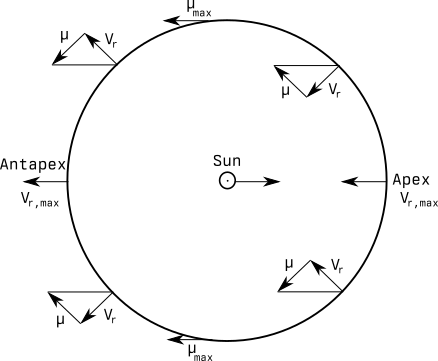
\includegraphics[width=0.5\textwidth]{static/solar_apex.png}
        \caption[The motion of the Sun in the LST.]
        {
          The motion of the Sun in the LST. The apex and antiapex are
          represented in the same and opposite direction of the Sun's motion.
          The combination of radial veolcities and proper motions of stars in the
          leads to the apparent motion of stars in the LST moving from the apex
          towards the antiapex.
        }
\label{fig:solar_apex}
\end{figure}

As the Sun progresses towards the solar apex, nearby stars appear to diverge
from this point in the celestial sphere. Conversely, stars seem to converge
towards each other in the direction of the solar antapex.

It is important to note that the Sun's motion within the Milky Way galaxy is not
solely restricted to the galactic plane; it also entails an oscillatory movement
relative to the plane spanning millions of years.

Authors like \cite{marceta2023} consider the role of the solar apex when
generating a synthetic population of interstellar objects in the solar system.
Figure \ref{fig:distribution_interlopers} shows the expected distribution of
interlopers.

\vspace{1cm}

\begin{figure}[H]
  \centering
  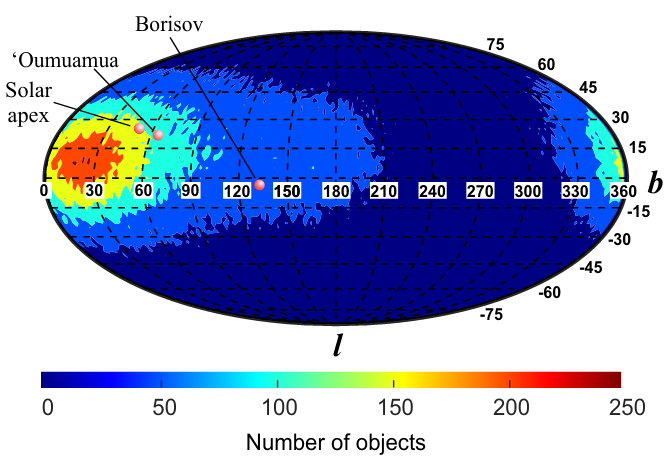
\includegraphics[width=0.9\textwidth]{static/distribution_interlopers.png}
        \caption[Expected interlopers distribution in the solar system.]{The
        expected distribution of interlopers in the solar system, represented in
        a galactic coordinates. A higher density of interlopers is expected in
        the direction of the solar apex. The direction of 'Oumuamua and Borisov
        is found to be close to this point, located near constellation Lyra.
        This contour plot is figure 11 of \cite{marceta2023} article. It is
        reproduced under permission of its original author.
        }
  \label{fig:distribution_interlopers}
\end{figure}

Despite this preferred direction, it is important to remember that there is
nothing that prevents and ISO to be discovered in other direction. In fact,
probabilities for intetifying an interloper approaching in the direction of the
solar-antapex are lower, but not null.

% https://iopscience.iop.org/article/10.3847/2041-8213/aaae67/meta

% Interstellar objects and exocomets: https://arxiv.org/pdf/2303.17980.pdf


\chapter{Revisiting targeting missions}

In this section, a review on targeting for space missions is presented. The
Lambert's problem is revisited together with its big role in targeting. Next,
the mathematical model used for this work is exposed. Finally, various mission
constrains are collected to showcase the challenged when planning a mission.

\section{Lambert's problem}

Lambert's problem is the boundary value problem (BVP) in the context of the
restricted two-body problem dynamics. Equation \ref{eq:lambert-bvp} models this
problem and figure \ref{fig:lambert-geometry} depicts its geometry.

\begin{equation}
  \ddot{\vec{r}} = -\frac{\mu}{r^3}\vec{r} \quad \begin{cases}
    \vec{r}(t_1) = \vec{r}_1 \\
    \vec{r}(t_2) = \vec{r}_2 \\
    \Delta t = t_2 - t_1
  \end{cases}
  \label{eq:lambert-bvp}
\end{equation}

If the initial position vector $\vec{r}_1$ is the launch position at time
$t_1$ and vector $\vec{r}_2$ is the arrival position at time $t_2$,
then it is possible to find the targeting orbit required to transfer a
spacecraft between the two.

Consider the case where the spacecraft is launched from a planetary body, like
the Earth, and is intended to reach an interloper. The ephemeris (position over
time) of the central body and the interloper are known. These can be used as the
input parameters for solving Lamber's problem for a given time of flight.

The solution to the Lambert's problem returns the values of $\vec{v_1}$ and
$\vec{v_2}$. Since the positions vectors are known, the computed velocity
vectors complete the state vectors at launch and arrival.

Once the velocity vectors are obtained, their modulus can be used to compute for
the required $\Delta v$. This is the increment in the velocity that needs to be
achieved by the propulsion system in order to insert the spacecraft into the
desired targeting orbit.

\begin{figure}[H]
  \centering
  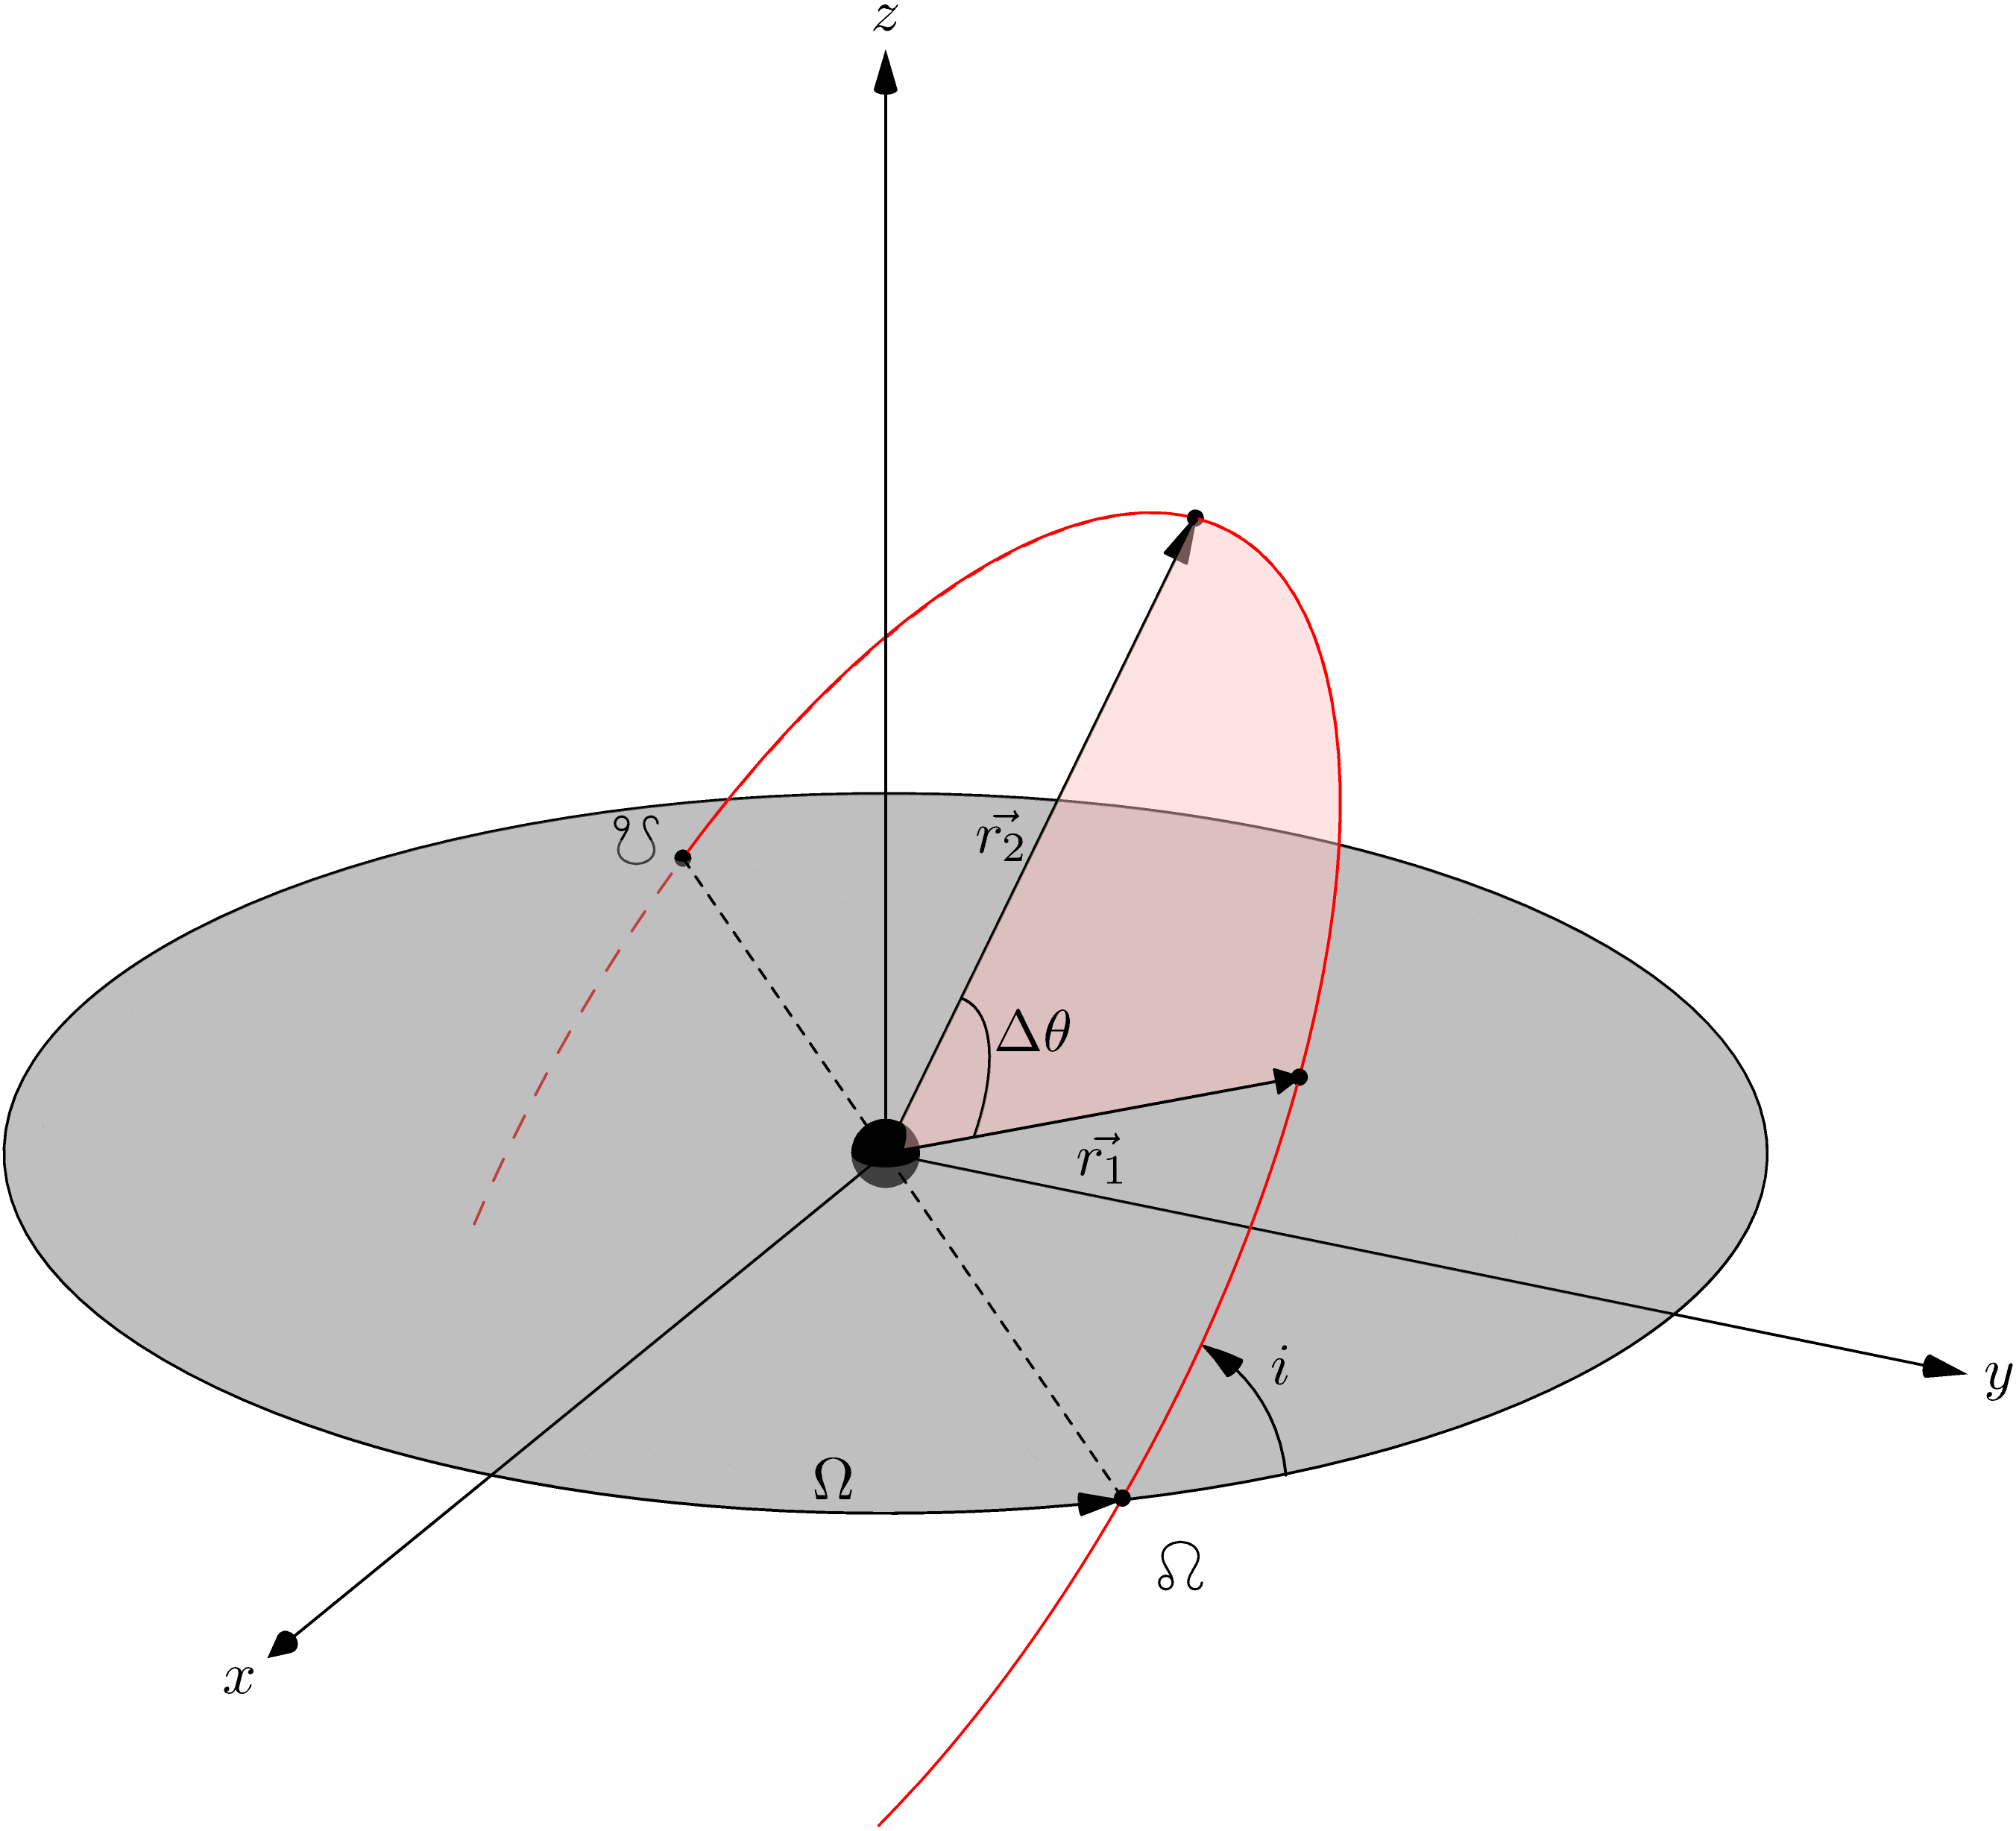
\includegraphics[width=0.75\textwidth]{lambert-problem/geometry.png}
  \caption{Lambert's problem geometry. The targeting orbit is represented by the red curve.}
  \label{fig:lambert-geometry}
\end{figure}

\subsection{Mathematical model}

Solving Lambert's problem requires numerical routines. Lots of algorithms have
been devised over the last century. The author of this document some of the most
popular ones and compared them in performance, see \cite{martinez2021}. Any
algorithm for solving Lambert's problem operates with the parameters presented
in table \ref{tab:lambert-parameters}.

\vspace{1cm}
\begin{table}[H]
  \centering
  \begin{tabular}{|c|c|}
    \hline
    Parameter   & Description                                             \\
    \hline
    $\mu$       & Gravitational parameter                                 \\
    $\vec{r}_1$ & Initial position vector                                 \\
    $\vec{r}_2$ & Final position vector                                   \\
    $\Delta t$  & Time of flight                                          \\
    $M$         & Number of desired revolutions                           \\
    Prograde    & Inclination of the final orbit                          \\
    Low path    & Type of path when more than two solutions are available \\
    Maxiter     & Maximum number of iterations when finding a solution    \\
    Atol        & Absolute tolerance of the numerical routine             \\
    Rtol        & Relative tolerance of the numerical routien             \\
    \hline
  \end{tabular}
  \caption{Parameters accepted by any Lambert's problem solver}
  \label{tab:lambert-parameters}
\end{table}

This work assumes Lambert's problem in the context of the restricted two-body
problem. This means that the only body exherting a gravitational influence is
the Sun. Thus, planetary bodies and interlopers are modeled as points with zero
mass and volume. Their gravitational influence is considered negligible, being
the only massive body the Sun. The required $\Delta v$ is modeled as an impulse.
This means that the change in the velocity is instantaneous. Perturbations are
not considered neither.

By sacrifying the accuracy of the model, the computational complexity of the
problem gets reduced. This reduces the time required to solve the problem.
Results obtained can be used as a first approximation for further refinement.

\section{Mission constraints}

% https://www.projectrho.com/public_html/rocket/infrastructure.php#eml1best

Despite simplifications, the mission design process is still a complex problem.
There exists a wide range of mission constraints that can be imposed on the
analysis to refine the results and make them more realistic. These include fuel
mass, characteristic energy, excess velocity at arrival, time of flight,
tracking constraints, and communication constraints. For a complete overview of
mission contraints, the reader is referred to \cite{smad2011}.

\subsection{Fuel mass}

The fuel mass is a critical constraint in mission design. For every impulse
performed by the spacecraft, a certain amount of fuel is consumed. This loss in
mass is modeled according to the Tsiolkovsky rocket equation \ref{eq:tsiolkovsky}:

\begin{equation}
        \Delta v = v_e \ln \left( \frac{m_0}{m_f} \right) = I_{sp} g_0 \ln \left( \frac{m_0}{m_f} \right)
        \label{eq:tsiolkovsky}
\end{equation}

Where $\Delta v$ is the change in velocity, $v_e$ is the exhaust velocity, $m_0$
is the initial mass of the spacecraft, $m_f$ is the final mass of the
spacecraft. Other variants of the expression include the $I_{sp}$, the specific
impulse of the propulsion system, and $g_0$, the standard gravity.

\subsection{Characteristic energy}

The characteristic energy $C_3$ is also a good estimator for the propulsion
requirements of a mission.

The $\Delta v$ relates with the characteristic energy $C_3$, also known as
specific energy. Equation \ref{eq:c3} summarizes this relation for hyperbolic
orbits:

\begin{equation}
        C_3 = v_{\infty}^2
        \label{eq:c3}
\end{equation}

Given a propulsion system, a maximum specific energy is imposed, limiting the
maximum $\Delta v$ that the spacecraft can achieve. If a spacraft can not reach
a certain characteristic energy, then the mission is not feasible and the
target orbit can not be achieved.

\subsection{Excess velocity at arrival}

Another mission constraint within the context of interlopers rendezvous is the
excess velocity at arrival. Lauch and arrival velocities are used to compute the
impulsed required to reach the target orbit. The first impulse $\Delta v_1$ is
used to launch the spacecraft into the target orbit. The second impulse $\Delta
v_2$ is used to adapt to the orbit of the interloper, leading to a rendezvous.
Thus, two scenarios are possible:

\begin{itemize}

    \item \textbf{Targeting of the interloper.} The spacecraft overshoots the target by
    not applying the final impulse. This ahieves a greater launch
    impulse as more fuel mass can be allocated for this task. However, the
    spacecraft is not able to rendezvous with the interloper, as the second
    impulse is never applied.

    \item \textbf{Rendezvous of the interloper.} The spacecraft performs the
    arrival impulse to adapt to the orbit of the interloper. This reduces the
    amount of fuel available for the launch impulse but allows the spacecraft to
    follow the interloper.

\end{itemize}

Wether the spacecraft overshoots the target or rendezvous with the interloper,
the excess velocity at arrival is a critical parameter.

\subsection{Time of flight}

The time of flight is another important constraint in mission design. It refers
to the elapsed time between the launch and the rendezvous with the interloper.
Usually, short times of flight are preferred. They reduce the exposure to space
radiaiton, which can affect the spacecraft and its electronics. However, short
time of flights require greater fuel mass and thus greater propulsion to achieve
greater speeds for covering the astronomical distances between the launch and
arrival positions.

\subsection{Tracking constraints}

The spacecraft must be able to track the interloper and its own position
relative to the stars background. By doing so, the spacecraft can assert if it
is on the right orbit and if it is following the interloper correctly.

However, tracking a small object in space is a challenging task. For example,
'Oumuamua did not presented any cometary activity, having an absolute magnitude
of $M = 22$ (JPL SBDB) which made it difficult to
observe and track it. On the other hand, Borisov exhibited a coma, making it
more visible by having a magnitude of $M = 16$, see \cite{jewitt2020}.

These constrains are not analyzed in this work, but they are important for the
success of the mission.

\subsection{Communication constraints}

Communication limits the reaction time of the spacecraft. Interlopers are
traveling at high speeds, and the spacecraft must be able to communicate along
astronomical distances.

\section{Direct orbit trasnfers}

This section presents the results computed for a direct orbit transfer between
Earth and the two interstellar objects. The analysis is performed by solving the
Lambert's problem under the Keplerian assumption. In addition, the modulus of the
escape velocity is added to the required launch velocity.

The algorithm used is the one presented by \cite{izzo2015}, as it is proven to
be more accurate and faster than other classical algorithms \cite{martinez2021}.
The ephemerides for 'Omuaumua and Borisov are obtained from JPL Horizons API
service at epoch January 1, 2018. These are propagated under the two-body
assumption to simplify the analysis. Maximum propagation date is January 1,
2035.

Porkchop plots for 'Oumuaumua and Borisov are shown in figure
\ref{fig:oumuamua-direct-transfer-porkchop} and figure
\ref{fig:borisov-direct-transfer-porkchop}. The limits for the characteristic
energy range between 0 and 12000 km$^2$/s$^2$.

\begin{figure}[H]
  \centering
  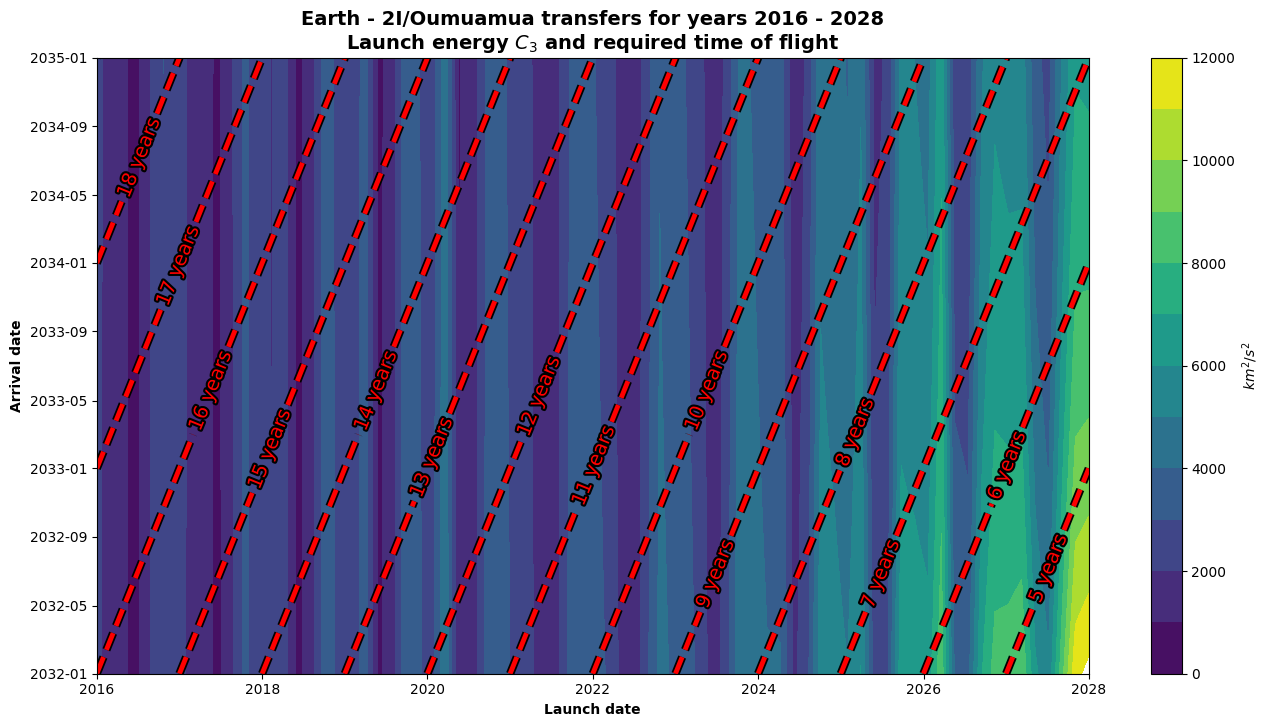
\includegraphics[width=\textwidth]{static/oumuamua/direct-transfer-porkchop.png}
  \caption{Launch energy porkchop plot for 1I/'Oumuamua.}
  \label{fig:oumuamua-direct-transfer-porkchop}
\end{figure}
\begin{figure}[H]
  \centering
  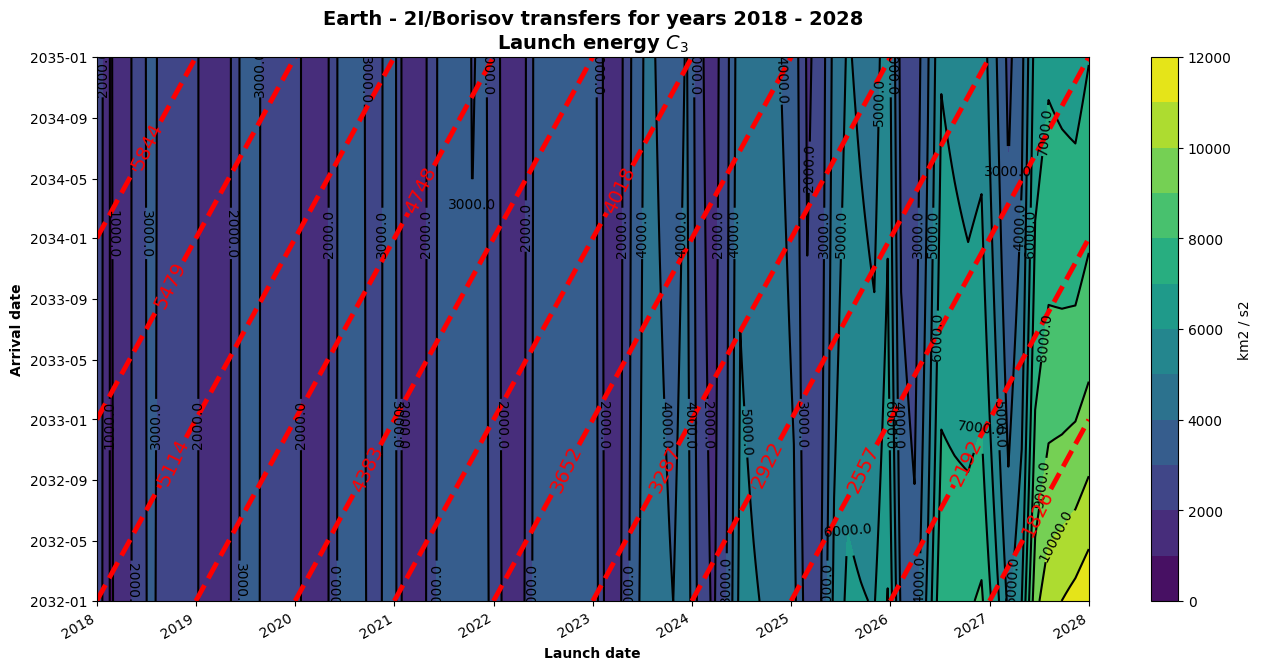
\includegraphics[width=\textwidth]{static/borisov/direct-transfer-porkchop.png}
  \caption{Launch energy porkchop plot for 2I/Borisov.}
  \label{fig:borisov-direct-transfer-porkchop}
\end{figure}

The contour maps show a periodic pattern, with a minimum energy transfer
corridor every year. This year corresponds to a more favorable position of the
Earth with respect to the interstellar object.

The most energy consuming area is located in the lower right corner of the plot.
This area corresponds to a shorter time of flight (4 years). The shorter the time of
flight, the greater the launch velocity and the energy required to perform the
transfer. On the other hand, the upper left corner corresponds to a longer time
of flight (17 years), with lower energy requirements.

It is worh noting that the energy required to reach 'Oumuamua is slightly lower
than the energy required to reach Borisov. This is due to the higher velocity of
this object, since 'Oumuamua is travelling at $26.0$ km/s whereas Borisov does
at $32.2$ km/s.

Finally, both porkchops show a similar contour map. This is due to the long
distance exhibited by the two interlopers in the future positions depicted in
the porkchop plot. The short-time transfer scenarios show differences between
'Oumuamua and Borisov, but the long-time transfer scenarios show close values.

\begin{figure}[H]
  \centering
  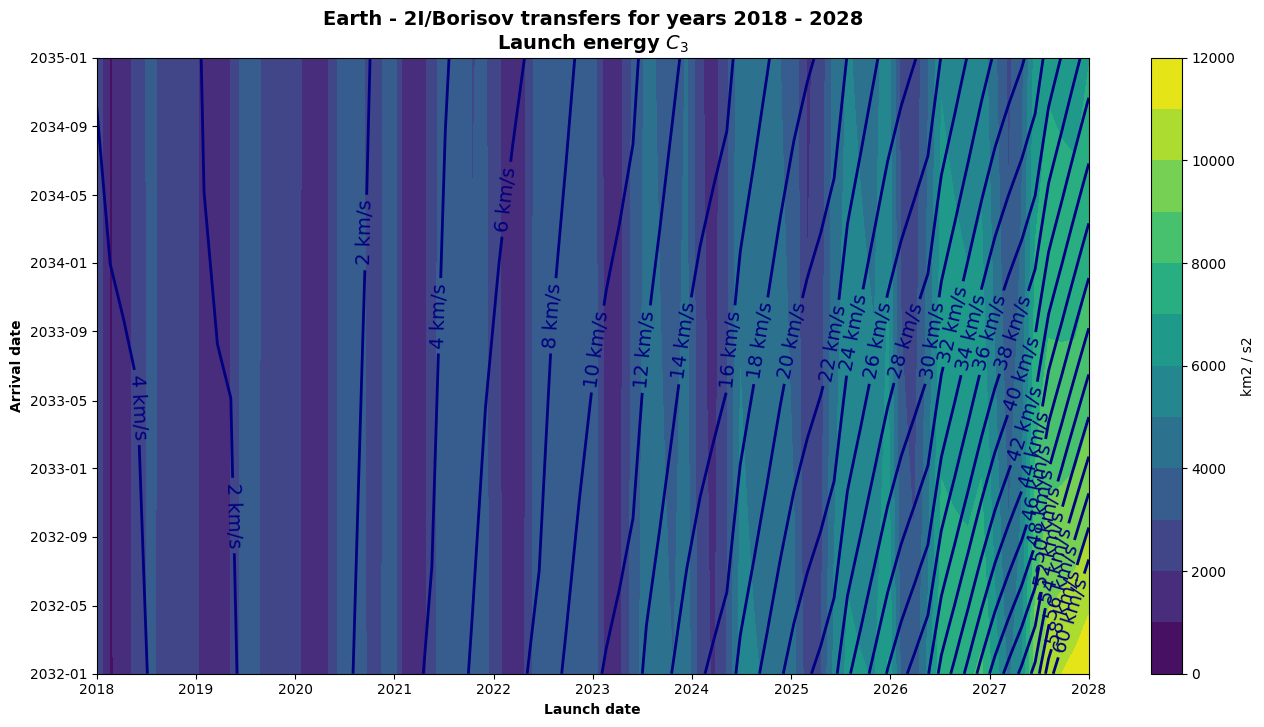
\includegraphics[width=\textwidth]{static/borisov/direct-transfer-porkchop-avl.png}
  \caption{Launch energy porkchop plot for 2I/Borisov.}
  \label{fig:oumuamua-direct-transfer-porkchop}
  \label{fig:borisov-direct-transfer-porkchop-avl}
\end{figure}




\chapter{Direct transfer analysis}

This chapter presents the direct transfer analysis performed on the two
discovered interstellar objects, 1I/'Oumuamua and 2I/Borisov. The analysis
includes porkchop plots for quickly visualizing different mission constraints.
The optimum transfers are represented graphically too. A short discussion on the
obtained values is presented at the end of the chapter.

\section{Porkchop plots analysis}

This section presents the results computed for a direct orbit transfer between
Earth and the two interstellar objects. The analysis is performed by solving the
Lambert's problem under the Keplerian assumption.

The algorithm used is the one devised by \cite{izzo2015}, as it is proven to be
more accurate and faster than other classical algorithms \cite{martinez2021}.
The ephemerides for 1I/'Omuaumua and 2I/Borisov are obtained from JPL Horizons
API service. These are propagated under the two-body assumption to simplify the
analysis. Propagation starts on January 1, 2016 and ends on January 1, 2035.

\subsection{Characteristic energy anslysis}

Porkchop plots for 'Oumuaumua and Borisov are shown in figure
\ref{fig:oumuamua-direct-transfer-porkchop} and figure
\ref{fig:borisov-direct-transfer-porkchop}. The limits for the characteristic
energy range between 0 and 12000 km$^2$/s$^2$. Isolines for the time of flight
are also included in these plots.

\newpage
\begin{figure}[H]
  \centering
  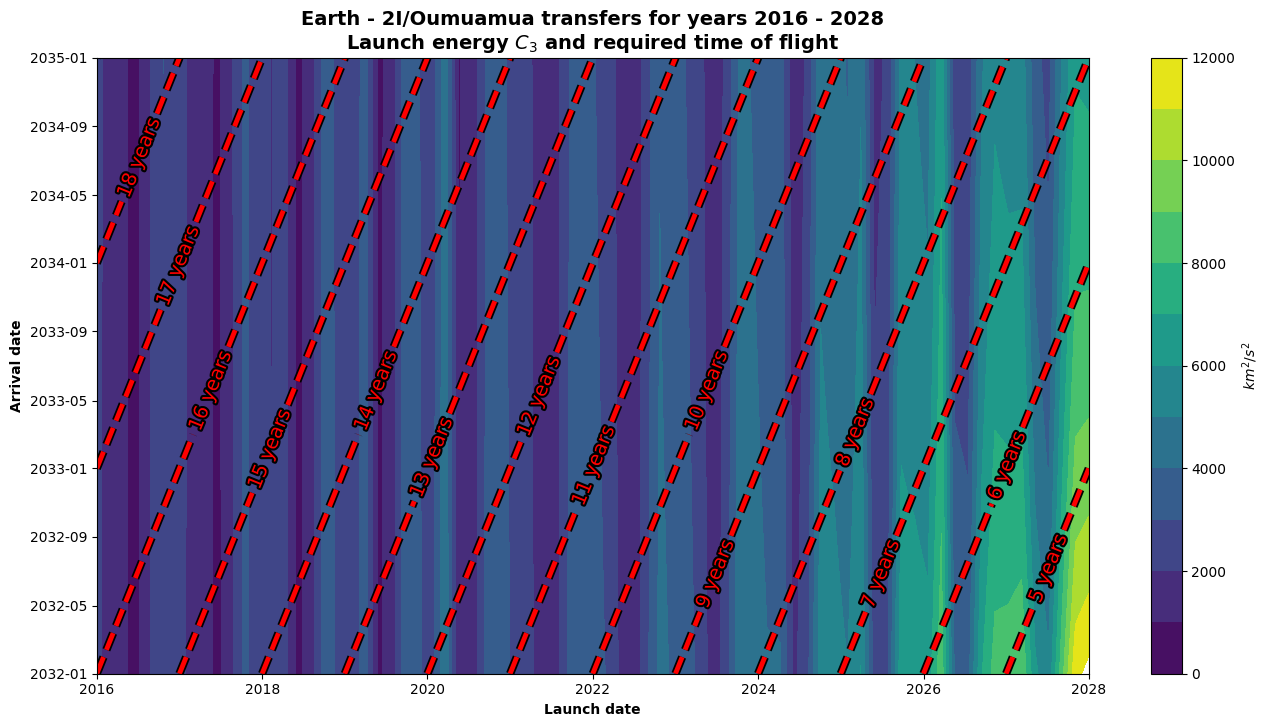
\includegraphics[width=\textwidth]{static/oumuamua/direct-transfer-porkchop.png}
  \caption{Launch energy porkchop plot for 1I/'Oumuamua.}
  \label{fig:oumuamua-direct-transfer-porkchop}
\end{figure}
\begin{figure}[H]
  \centering
  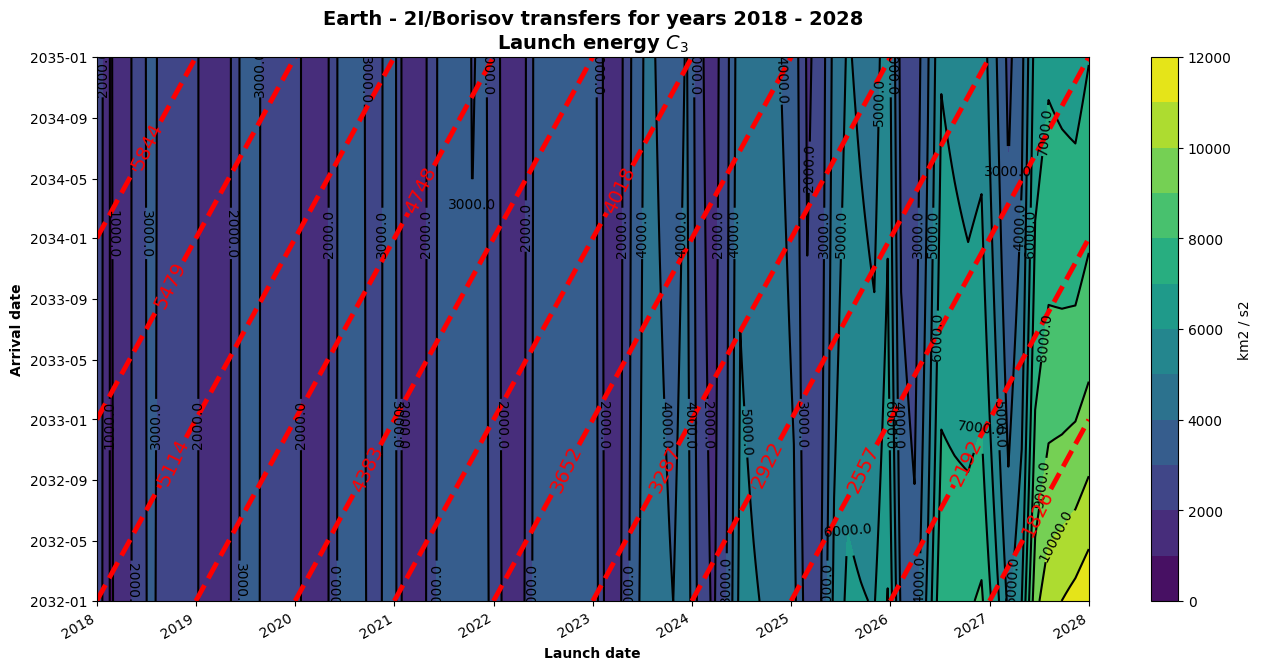
\includegraphics[width=\textwidth]{static/borisov/direct-transfer-porkchop.png}
  \caption{Launch energy porkchop plot for 2I/Borisov.}
  \label{fig:borisov-direct-transfer-porkchop}
\end{figure}
\newpage

The contour maps show a periodic pattern, with a minimum energy transfer
corridor every year. This year corresponds to a more favorable position of the
Earth with respect to the interstellar object.

The most energy consuming transfers are located in the lower right corner of the
plot. This area corresponds to a shorter time of flight (4 years). The shorter
the time of flight, the greater the launch velocity and the energy required to
perform the transfer. On the other hand, the upper left corner corresponds to a
longer time of flight (17 years), with lower energy requirements.

It is worh noting that the energy required to reach 'Oumuamua is slightly lower
than the energy required to reach Borisov. This is due to the higher velocity of
this object, since 'Oumuamua is travelling at $26.0$ km/s whereas Borisov does
at $32.2$ km/s.

Finally, both porkchops show a similar contour map. This is due to the long
distance exhibited by the two interlopers in the future positions depicted in
the porkchop plot. The short-time transfer scenarios show differences between
'Oumuamua and Borisov, but the long-time transfer scenarios show similar values.

\subsection{Arrival velocity analysis}

Figures \ref{fig:oumuamua-direct-transfer-porkchop-avl} and
\ref{fig:borisov-direct-transfer-porkchop-avl} show the isolines for the excess
arrival velocity. Values up to $24$ km/s are represented. Higher values may be
represented but they are not shown in the plots for graphic convenience.

The values are extraordinary high. Even if with a targeting mission (no second
impulse), the available observation time and coma samples capture would be
minimum. The direct rendezvous scenario seems unfeasible for nowadays
technology.

For 'Oumuamua, launch dates after 2022 lead to an excess arrival velocity
greater than $10$ km/s. For Borisov, any launch date after 2023 leads to the same
situation.

It is worth noting that the optimum dates for a lower closer to the discovery of
the interlopers. If a ready-to-launch mission would have been available, a quick
launch may have lead to a close targeting with these interplanetary objects.

\newpage
\begin{figure}[H]
  \centering
  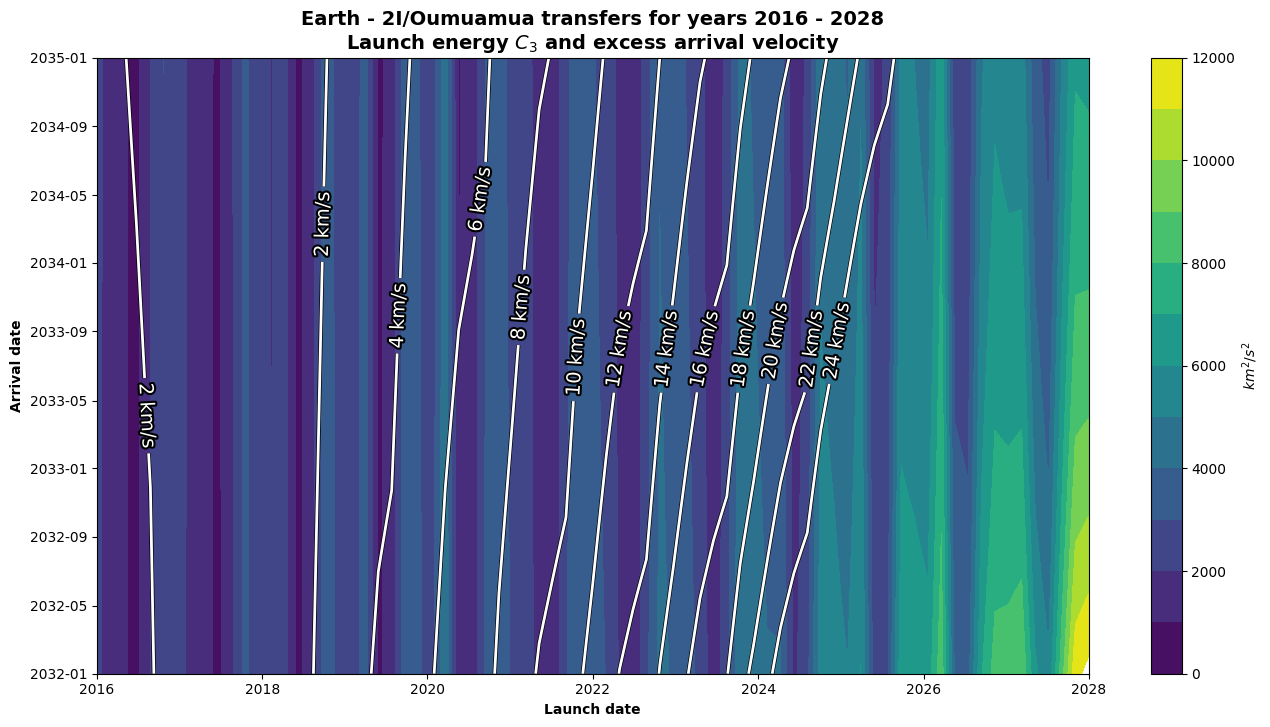
\includegraphics[width=\textwidth]{static/oumuamua/direct-transfer-porkchop-avl.png}
  \caption{Launch energy porkchop plot for 1I/'Oumuamua showing the isolines for
        excess arrival velocity. Compared to 2I/Borisov, a rendezvous with
        'Oumuamua leads to more excess arrival velocity for the time of flight.}
  \label{fig:oumuamua-direct-transfer-porkchop-avl}
\end{figure}
\begin{figure}[H]
  \centering
  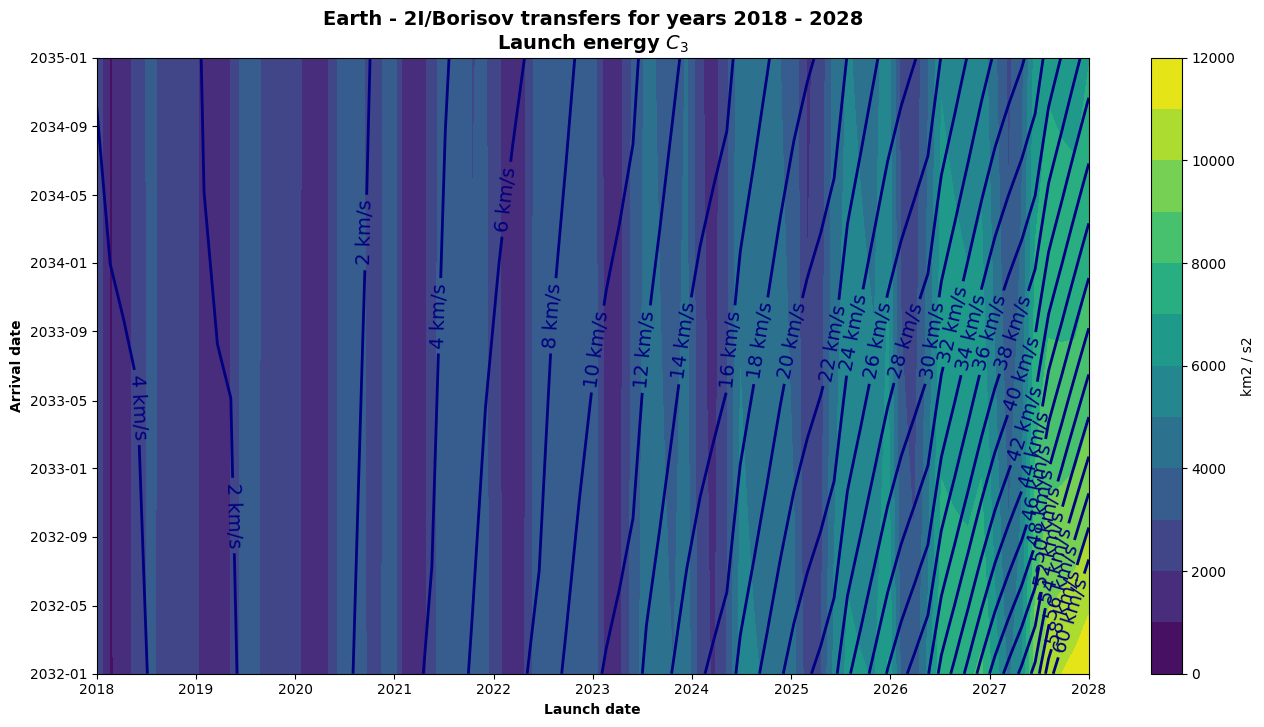
\includegraphics[width=\textwidth]{static/borisov/direct-transfer-porkchop-avl.png}
  \caption{Launch energy porkchop plot for 2I/Borisov showing the isoliens for
        excess arrival velocity. The shorter the flight of time, the greater the
        excess arrival velocity. Values are minimized for a transfer close to
        the discovery of the object.}
  \label{fig:borisov-direct-transfer-porkchop-avl}
\end{figure}
\newpage


\chapter{Alternate transfers}

After the results obtained in section \ref{sec:direct-results}, it is possible
now to study the possibility of using alternate transfers. The main goal of this
second analysis is to find a suitable transfer that is less expensive than a
direct transfer from the Earth. For this purpose, the following scenarios are
considered: orbits launching from a Lagrange point and gravity assisted
maneuvers.


\section{Lagrange points analysis}
\label{sec:lagrange-points-analysis}

Lagrangian points are a set of special locations in the vicinity of two massive
bodies where a small object will maintain a relatively stable position relative
to the two massive bodies. The five Lagrange points are labeled L1 through L5.
L1, L2, and L3 are collinear with the two massive bodies, while L4 and L5 are
located at the vertices of the equilateral triangle formed by the two massive
bodies. The L1, L2, and L3 points are unstable, while L4 and L5 are stable. The
L4 and L5 points are sometimes called Trojan points, and the two massive bodies
are sometimes called the primaries. Figure \ref{fig:lagrange_points} shows the
Lagrange points in the Sun - Earth-Moon barycenter system.

Despite L1, L2, and L3 being unstable, they are of particular interest because
of their proximity to the primaries. In fact, stable orbits can be achieved
by performing small corrections to the spacecrafts's position. Also, these
points are not populated with asteroids like L4 and L5, making them excellent
for long term missions.

In this work, only the point L2 belonging to the Sun - Earth system is
considered. The reason for choosing this point is that it is a popular point
chosed by different missions and thus, a well known point. It provides a great
viewpoint. In fact, this point has been selected for other missions including
the James Webb Space Telescope, see \cite{gardner2006}, or the future Comet
Interceptor, see \cite{jones2019}.

\begin{figure}[H]
  \centering
  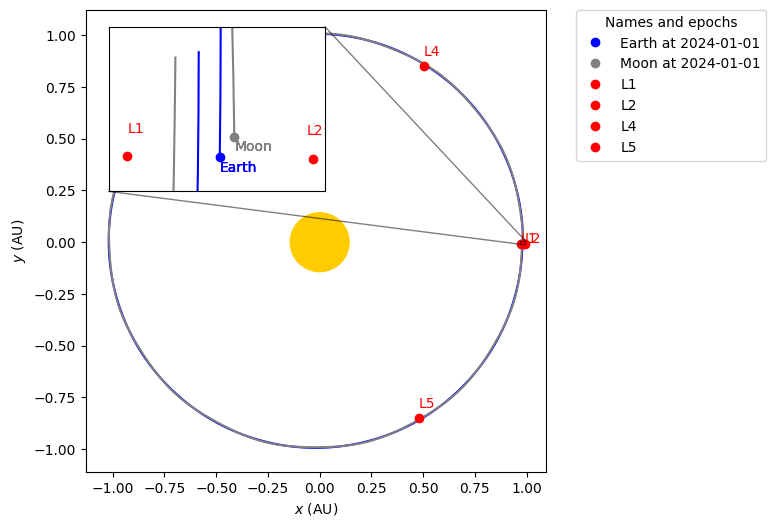
\includegraphics[width=\textwidth]{static/lagrange_points.png}
  \caption[Lagrange points in the Sun - Earth system.]{Lagrange points in the
    Sun - Earth-Moon barycenter system. All points are shown except L3. Ephemerides for this
    point are not provided by the JPL Horizons system. Despite this
    situation, the point is not analyzed in this work.}
  \label{fig:lagrange_points}
\end{figure}

\subsection{Escape velocity from L2}

For the computation of the escape velocity in the vicinity of the Lagrange
points, the gravitation effects of the Earth and the Moon are considered. Even
if the Lagrange points only appear in the restricted three-body problem,
computing the escape velocity requires using the two-body problem is still a
valid approach as long as the barycenter of the Earth-Moon system is used.

Thus, the escape velocity can be computed using equation \ref{eq:escape_velocity}.

\begin{equation}
  v_{\text{esc}} = \sqrt{\frac{2 \mu}{d}} = \sqrt{\frac{2 \mu}{\norm{\vec{r_b} - \vec{r}}}}
  \label{eq:escape_velocity}
\end{equation}

where in $\mu$ is the gravitational parameter of the Earth-Moon system, and $d$
is the distance from the point of interest to the barycenter of the Earth-Moon
system, which can be computed using equation \ref{eq:earth_moon_distance}.

\begin{equation}
  \vec{r_{b}} = \frac{\vec{r_{\text{\Terra}}} \cdot m_{\text{\Terra}}
    + \vec{r_{\text{\Moon}}} \cdot m_{\text{\Moon}}}{m_{\text{\Terra}} +
    m_{\text{\Moon}}}
  \label{eq:earth_moon_distance}
\end{equation}

To simplify the computer routines, an average value for the escape velocity has
been computed by solving previous equations for a span of time ranging between
years 2000 and 2050. The mean value for the escape velocity from L2 is $0.73$
km/s.

\subsection{Optimum direct transfers from L2}

The analysis for a direct optimum transfer from L2 to each one of the discovered
ISOs follows the same model than the one presented in chapter
\ref{ch:direct-transfer}.

\subsubsection{'Oumuamua}

Figures \ref{fig:l2-oumuamua-optimum-porkchop} and
\ref{fig:l2-oumuamua-optimum-porkchop-avl} show the porkchop plots showing the
launch energy, time of flight, and arrival velocity for a direct prograde launch
between L2 and 'Oumuamua.

\begin{figure}[H]
  \centering
  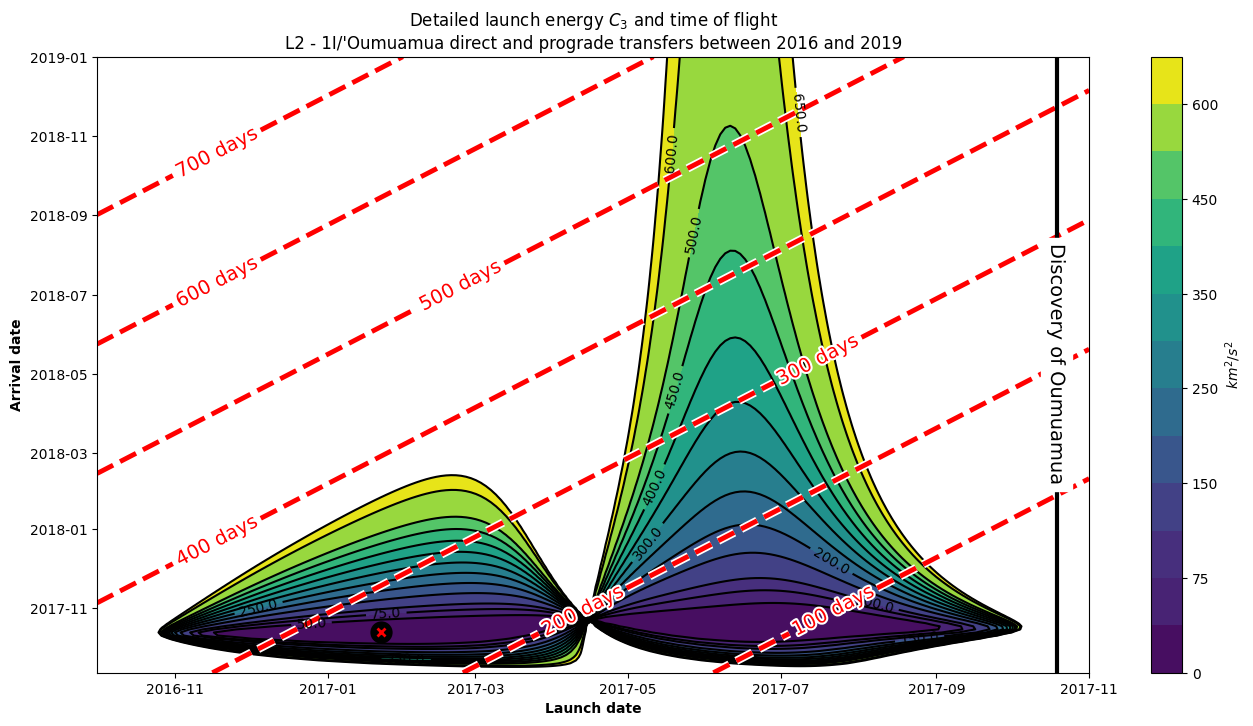
\includegraphics[width=\textwidth]{static/oumuamua/l2-direct-detailed-porkchop-tof.png}
  \caption[Detailed porkchop showing the optimum transfer for
    L2 to 1I/'Oumuamua with the time of flight.]{Detailed porkchop showing the optimum transfer for
    L2 to 1I/'Oumuamua.
  }
  \label{fig:l2-oumuamua-optimum-porkchop}
\end{figure}

Note that these figures are very similar to the ones in
\ref{fig:oumuamua-optimum-porkchop} and \ref{fig:oumuamua-optimum-porkchop-avl}.
The main difference is that launching from L2 requires less fuel, since the
escape velocity is lower. The required launch energy reduces about 92.81\%.
Despite this advantage, the arrival velocity is still high. Launch and arrival
dates are shown in table \ref{tab:l2-oumuamua-direct-transfer-optimum}.

\begin{figure}[H]
  \centering
  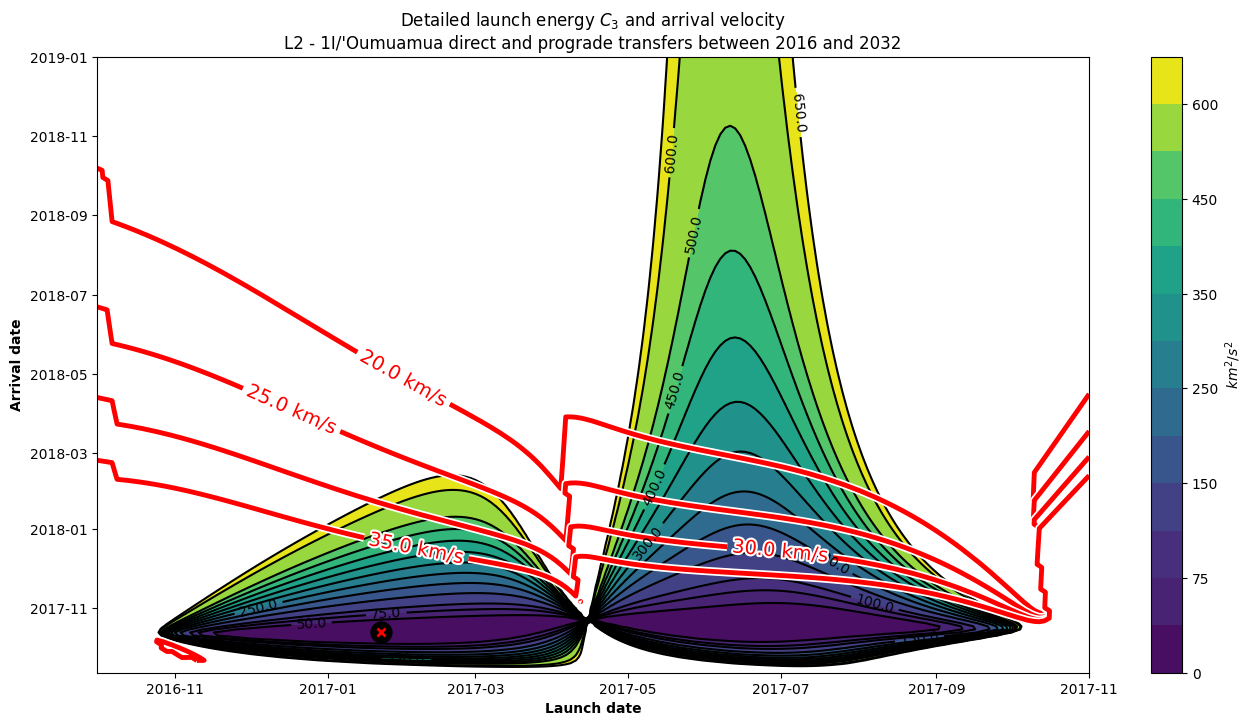
\includegraphics[width=\textwidth]{static/oumuamua/l2-direct-detailed-porkchop-avl.png}
  \caption[Detailed porkchop showing the optimum transfer for
    L2 to 1I/'Oumuamua with the arrival velocity.]{Detailed porkchop showing the
    optimum transfer for L2 to 1I/'Oumuamua with isolines for the arrival
    velocity.}
  \label{fig:l2-oumuamua-optimum-porkchop-avl}
\end{figure}

\vspace{1cm}
\begin{table}[H]
  \centering
  \begin{tabular}{|c|c|c|c|}
    \hline
    Object       & Launch date & Arrival date & Required $C_3$ [km$^2$/s$^2$] \\
    \hline
    1I/'Oumuamua & 2017-01-22  & 2017-10-13   & 14.41                         \\
    \hline
  \end{tabular}
  \caption[Optimum transfer orbit for a direct transfer between L2 and
    1I/'Oumuamua.]{Optimum transfer orbit for a direct transfer between
    L2 and 1I/'Oumuamua. The energy includes the required impulse for
    escaping the L2 point and for performing a targeting maneuver.}
  \label{tab:l2-oumuamua-direct-transfer-optimum}
\end{table}

The optimum transfer orbit is found to have a time of flight $\Delta t = 263.67$
days. The total cost of the launch is $\Delta v_\text{launch} = \Delta v_e +
  \Delta v_1 = 0.73 \text{ km/s} + 3.07 \text{ km/s} = 3.80$ km/s. The arrival
impulse is $\Delta v_2 = 61.46$ km/s. If the rendezvous is considered, the total
cost of the maneuver adds up to $\Delta v = 64.53$ km/s. Detailed impulses are
shown in table \ref{tab:l2-oumuamua-direct-transfer-impulses}.

\vspace{1cm}
\begin{table}[H]
  \centering
  \begin{tabular}{|c|c|c|c|}
    \hline
    Impulse & $\Delta v_x$ [km/s] & $\Delta v_y$ [km/s] & $\Delta v_z$ [km/s] \\
    \hline
    Launch  & 1.67                & -1.30               & 2.21                \\
    \hline
    Arrival & 58.04               & -14.06              & 14.47               \\
    \hline
  \end{tabular}
  \caption[Required impulses for a direct prograde transfer between L2 and
    'Oumuamua]{Required impulses for a direct prograde transfer between L2 and
    'Oumuamua.}
  \label{tab:l2-oumuamua-direct-transfer-impulses}
\end{table}


\subsubsection{Borisov}

Figures \ref{fig:l2-borisov-optimum-porkchop} and
\ref{fig:l2-borisov-optimum-porkchop-avl} show the porkchop plots showing the
launch energy, time of flight, and arrival velocity for a direct prograde launch
between L2 and Borisov.

\begin{figure}[H]
  \centering
  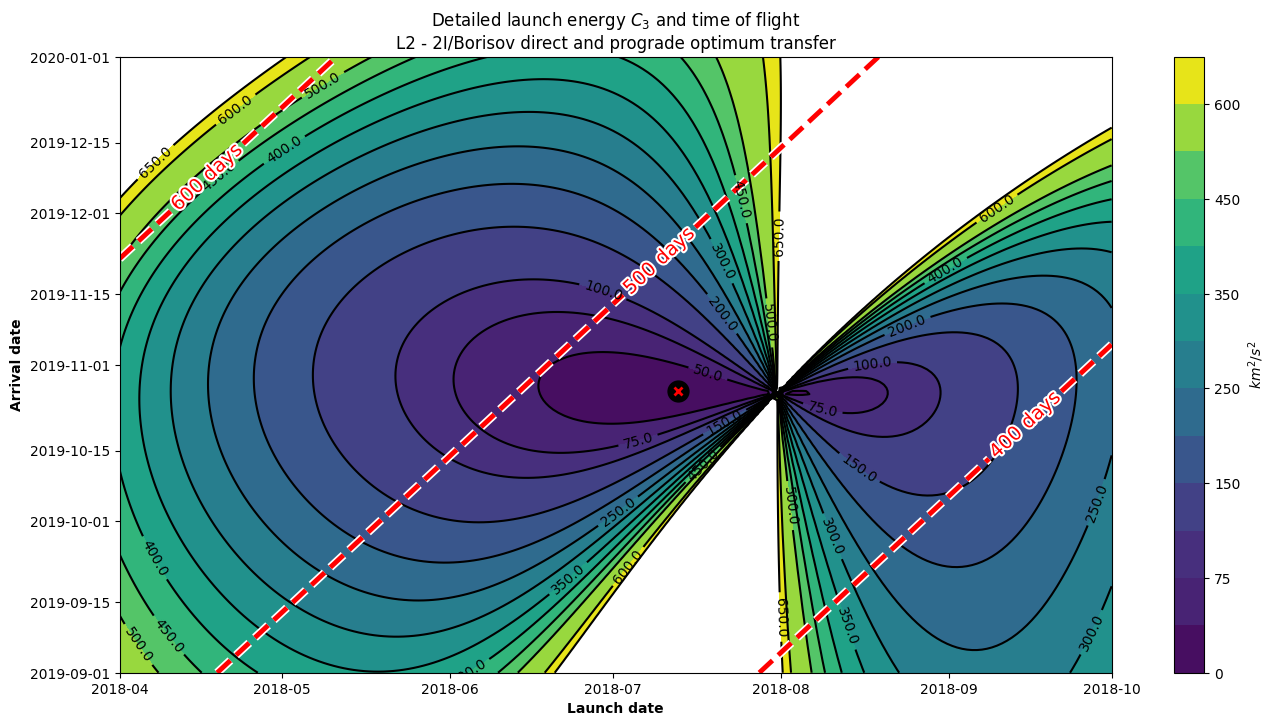
\includegraphics[width=\textwidth]{static/borisov/l2-direct-detailed-porkchop-tof.png}
  \caption[Detailed porkchop showing the optimum transfer for
    L2 to 2I/Borisov with the time of flight.]{Detailed porkchop showing the optimum transfer for
    L2 to 2I/Borisov. A point under 50 km$^2$/s$^2$ is found, highly
    reducing the launch cost from this Lagrange point.
  }
  \label{fig:l2-borisov-optimum-porkchop}
\end{figure}

\begin{figure}[H]
  \centering
  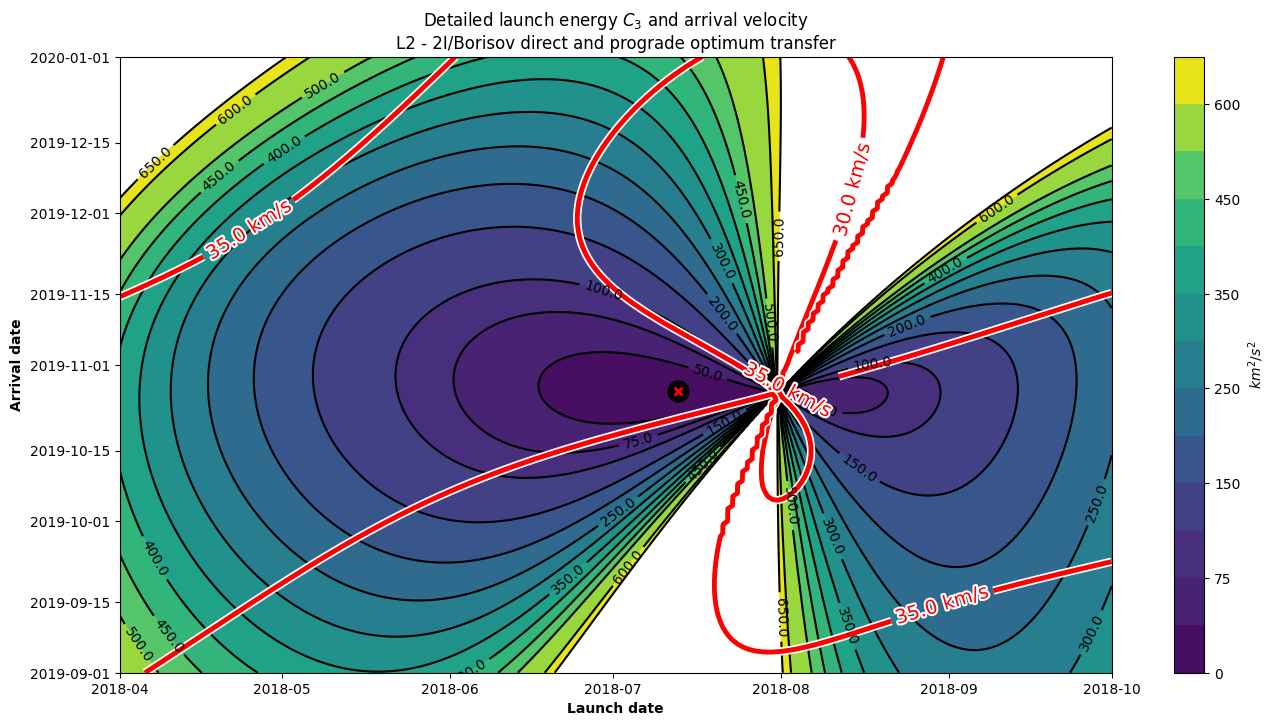
\includegraphics[width=\textwidth]{static/borisov/l2-direct-detailed-porkchop-avl.png}
  \caption[Detailed porkchop showing the optimum transfer for
    L2 to 2I/Borisov with the arrival velocity.]{Detailed porkchop showing the
    optimum transfer for L2 to 2I/Borisov with isolines for the arrival
    velocity. The optimum transfer point is found to have an arrival speed
    close to 33 km/s.}
  \label{fig:l2-borisov-optimum-porkchop-avl}
\end{figure}

Again, these figures are very similar to the ones in
\ref{fig:borisov-optimum-transfer-porkchop-tof} and
\ref{fig:borisov-optimum-transfer-porkchop-avl}. Again, launching from L2
requires less fuel. The required launch energy reduces about 88.08\%, yet the
arrival velocity is still high. Launch and arrival dates are shown in table
\ref{tab:l2-borisov-direct-transfer-optimum}.

\vspace{1cm}
\begin{table}[H]
  \centering
  \begin{tabular}{|c|c|c|c|}
    \hline
    Object     & Launch date & Arrival date & Required $C_3$ [km$^2$/s$^2$] \\
    \hline
    2I/Borisov & 2018-07-12  & 2019-10-26   & 34.30                         \\
    \hline
  \end{tabular}
  \caption[Optimum transfer orbit for a direct transfer between L2 and
    2I/Borisov.]{Optimum transfer orbit for a direct transfer between
    L2 and 2I/Borisov. The energy includes the required impulse for
    escaping the L2 point and for performing a targeting maneuver.}
  \label{tab:l2-borisov-direct-transfer-optimum}
\end{table}

The optimum transfer orbit is found to have a time of flight $\Delta t = 470.79$
days. The total cost of the launch is $\Delta v_\text{launch} = \Delta v_e +
  \Delta v_1 = 0.73 \text{ km/s} + 5.13 \text{ km/s} = 5.83$ km/s. The arrival
impulse is $\Delta v_2 = 33.02$ km/s. If the rendezvous is considered, the total
cost of the maneuver adds up to $\Delta v = 38.85$ km/s. Detailed impulses are
shown in table \ref{tab:l2-borisov-direct-transfer-optimum}.

\vspace{1cm}
\begin{table}[H]
  \centering
  \begin{tabular}{|c|c|c|c|}
    \hline
    Impulse & $\Delta v_x$ [km/s] & $\Delta v_y$ [km/s] & $\Delta v_z$ [km/s] \\
    \hline
    Launch  & 4.82                & 1.71                & 0.30                \\
    \hline
    Arrival & -1.61               & -18.34              & -27.42              \\
    \hline
  \end{tabular}
  \caption[Required impulses for a direct prograde transfer between L2 and
    Borisov]{Required impulses for a direct prograde transfer between L2 and
    Borisov.}
  \label{tab:l2-borisov-direct-transfer-impulses}
\end{table}

\subsubsection{Summary}

Results obtained for the direct transfers from L2 to 1I/'Oumuamua and 2I/Borisov
not only demonstrate significant reductions in launch energy but also underscore
the strategic advantage of positioning a spacecraft at the Lagrange point L2. By
parking a spacecraft at L2, the mission can leverage its stable orbit and
gravitational equilibrium, effectively establishing a strategic vantage point
for interstellar rendezvous. This positioning provides invaluable reaction time,
enabling meticulous planning and adjustment of trajectory parameters before
initiating the final approach toward the target object.


\chapter{Conclusions}

After the direct transfer analysis from Earth in \ref{ch:direct-transfer}, the
direct transfer analysis from L2 in \ref{sec:lagrange-points-analysis}, and a
the gravity assist review in \ref{sec:gravity-assist-analysis}, this chapter
sumarizes all the results and presents the final conclusions.

\section{Optimum direct transfer: Earth vs L2}

Results for the optimum direct transfer computed previous chapters are
summarized in tables \ref{tab:summary-results-v-launch},
\ref{tab:summary-results-c3-launch} and \ref{tab:summary-results-arrival-v}. A
high reduction in the launch energy is observed when launching from L2 instead
of Earth. This reduction is mainly due to the low escape velocity at L2, which
allows for a more efficient transfer.

\vspace{1cm}
\begin{table}[H]
  \centering
  \begin{tabular}{|c|c|c|c|}
    \hline
    Object       & $\Delta v$ launch Earth [km/s] & $\Delta v$ launch L2 [km/s] & Reduction [\%] \\
    \hline
    1I/'Oumuamua & 13.85                          & 3.80                        & 72.56          \\
    \hline
    2I/Borisov   & 16.90                          & 5.85
                 & 65.38                                                                         \\
    \hline
  \end{tabular}
  \caption[Comparison of the launch velocity for direct transfers from Earth and
    L2.]{Comparison of the launch velocity for direct transfers from Earth and
    L2. These values are feasible considering modern propulsion technology,
    see \cite{longhurst2021}.}
  \label{tab:summary-results-v-launch}
\end{table}

\vspace{1cm}
\begin{table}[H]
  \centering
  \begin{tabular}{|c|c|c|c|}
    \hline
    Object       & $C_3$ launch Earth [km$^2$/s$^2$] & $C_3$ launch L2 [km$^2$/s$^2$] & Reduction [\%] \\
    \hline
    1I/'Oumuamua & 192.00                            & 14.41                          & 92.51          \\
    \hline
    2I/Borisov   & 286.00                            & 34.30                          & 88.08          \\
    \hline
  \end{tabular}
  \caption[Comparison of the launch energy for direct transfers from Earth and
    L2.]{Comparison of the launch energy for direct transfers from Earth and L2. A reduction in energy is observed when launching from L2.}
  \label{tab:summary-results-c3-launch}
\end{table}

\vspace{1cm}
\begin{table}[H]
  \centering
  \begin{tabular}{|c|c|c|c|}
    \hline
    Object       & $\Delta V$ arrival Earth [km/s] & $\Delta V$ arrival L2 [km/s] & Reduction [\%] \\
    \hline
    1I/'Oumuamua & 62.33                           & 61.46                        & 1.40           \\
    \hline
    2I/Borisov   & 33.00                           & 33.02                        & -0.06          \\
    \hline
  \end{tabular}
  \caption[Comparison of the arrival velocity for direct transfers from Earth and
    L2.]{Comparison of the arrival velocity for direct transfers from Earth and
    L2. Due to the close proximity of L2 to the Earth, the reduction in
    arrival speed is low compared to the reduction in launch energy.}
  \label{tab:summary-results-arrival-v}
\end{table}




Note that the required $\Delta v$ values for a transfer originating at L2 can be
achieved with modern propulsion technology and gravitational assists. However,
this research considers the usage of impulsive maneuvers, that is, maneuvers
that occur instantaneously. In reality, the spacecraft would need to perform
a maneuver over a period of time. Not only this, figure \ref{fig:payload_vs_c3}
only considers main space launchers, which are used for launching satellites.

For a spacecraft placed at L2, a bipropellant chemical propulsion system, such
as one using liquid oxygen and liquid hydrogen or liquid oxygen and liquid
ethanol, would be a feasible option to provide the required 3.5 km/s of $\Delta
  v$. The high specific impulse of bipropellant systems makes them capable of
delivering this level of performance.

Leveraging the advantageous position of L2 not only facilitates spacecraft
parking while awaiting the discovery of new ISOs but also augments mission
adaptability. By pre-positioning a spacecraft in space, it affords greater
maneuverability and flexibility in mission planning. This positioning grants
extended reaction time, enabling meticulous mission strategizing and the
optimization of trajectory paths.

Tables \ref{tab:optimum-launch-dates-oumuamua} and
\ref{tab:optimum-launch-dates-borisov} summary the optimum launch dates for
1I/'Oumuamua and 2I/Borisov, respectively. It is worth mentioning that the
optimum launch dates for 1I/'Oumuamua and 2I/Borisov take place before humanity
discovered them. This fact highlights the importance of increasing the
investment in space surveillance and tracking systems. By doing so, the reaction
time to intercept an ISO could be reduced significantly, allowing for more
efficient missions.

\vspace{1cm}
\begin{table}[H]
  \centering
  \begin{tabular}{|c|c|c|c|}
    \hline
    Object       & Optimum date launch Earth & Optimum date launch L2 & Discovery date \\
    \hline
    1I/'Oumuamua & 2017-01-20                & 2017-01-22             & 2017-10-19     \\
    \hline
  \end{tabular}
  \caption[Optimum launch dates for 1I/'Oumuamua compared to discovery its
    discovery date]{Optimum launch dates for
    1I/'Oumuamua compared to its discovery date. The first interstellar
    interloper was discovered close to 270 days after an optimum transfer
    could have been launched from Earth or L2.}
  \label{tab:optimum-launch-dates-oumuamua}
\end{table}

\vspace{1cm}
\begin{table}[H]
  \centering
  \begin{tabular}{|c|c|c|c|}
    \hline
    Object     & Optimum date launch Earth & Optimum date launch L2 & Discovery date \\
    \hline
    2I/Borisov & 2018-07-12                & 2018-07-12             & 2019-08-30     \\
    \hline
  \end{tabular}
  \caption[Optimum launch dates for 2I/Borisov compared to discovery its
    discovery date]{Optimum launch dates for
    2I/Borisov compared to its discovery date. The second interstellar
    interloper was discovered close to 414 days after an optimum transfer
    could have been launched from Earth or L2.}
  \label{tab:optimum-launch-dates-borisov}
\end{table}

\section{About gravity assists}

Regarding the analysis of gravity assists, it is determined that their
feasibility hinges on several factors. These encompass the relative spatial
configurations of planets during the launch phase, the duration of the mission,
the inclination concerning the ecliptic plane of the ISO, the velocity of the
interloper, and the launch velocity itself. In scenarios ripe with optimism, the
feasibility of executing multiple gravity assists, possibly involving inner
planets, emerges as a promising prospect.

These results mirror the strategic approach undertaken by the Comet Interceptor
mission. The mission advocates for the adoption of a direct external transfer
orbit from L2 in a ready-to-launch state to the interloper, presenting it as an
initial solution to surmount the intricacies associated with interplanetary
transfer challenges.

\section{Future work}

While working on this project, the author noticed a lack of robust software for
optimizing gravity assist trajectories. Trajectory optimization in astrodynamics
is complex, especially when dealing with multiple planetary flybys and impulsive
maneuvers.

Creating software to optimize gravity assist trajectories considering variables
like planetary configurations, time spans, and fuel constraints would be highly
beneficial. Such software could quickly design an optimal mission to intercept
an interstellar visitor, helping astrodynamicists overcome challenges like high
relative speeds and inclinations.


% ----------- END OF CONTENT FILES -------------


% Cite the bibliography
\printbibliography

\end{document}
